\chapter{Búsqueda binaria}

\section{Planetas}
Tienes un conjunto de planetas y te dan las posiciones de estos planetas, quieres colocar un meteorito en cualquier lugar entre los planetas, el meteorito debe quedarse en su lugar y no ser atraido por la fuerza gravitacional de los planetas. 
Sabemos de física básica que la sumatoria de todas las fuerzas debe ser igual con cero. Sabemos que:
\begin{itemize}
    \item $F_{1} = F_{2}$ esta en equilibrio el sitema
    \item $F_{1} > F_{2}$
    \item $F_{1} < F_{2}$
\end{itemize}

Tenemos como información la siguiente fórmula:
\[
    \frac{1}{|X_{i} - M|}    
\]

Ejemplo:
\begin{figure}[H]
    \begin{center}
    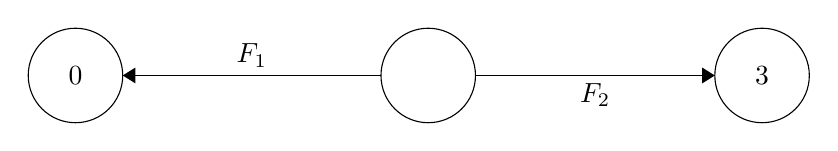
\begin{tikzpicture}[scale=0.2]
    \tikzstyle{every node}+=[inner sep=0pt]
    \draw [black] (18.7,-25.1) circle (3);
    \draw (18.7,-25.1) node {$0$};
    \draw [black] (62.3,-25.1) circle (3);
    \draw (62.3,-25.1) node {$3$};
    \draw [black] (41.1,-25.1) circle (3);
    \draw [black] (38.1,-25.1) -- (21.7,-25.1);
    \fill [black] (21.7,-25.1) -- (22.5,-25.6) -- (22.5,-24.6);
    \draw (29.9,-24.6) node [above] {$F_{1}$};
    \draw [black] (44.1,-25.1) -- (59.3,-25.1);
    \fill [black] (59.3,-25.1) -- (58.5,-24.6) -- (58.5,-25.6);
    \draw (51.7,-25.6) node [below] {$F_{2}$};
    \end{tikzpicture}
    \end{center}
\end{figure}

Si utilizamos las fórmulas calculamos el valor de $F_{1}, F_{2}$
\[
    F_{1} = \frac{1}{|0 - 1.5|} = \frac{1}{1.5}    
\]
y
\[
    F_{2} = \frac{1}{|3 - 1.5|} = \frac{1}{1.5}    
\]

Podemos ver que si restamos ambas fuerzas efectivamente el sistema está en equilibrio.

Pero ¿Qué pasa si tenemos más de dos planetas? Tenemos n - 1 soluciones ya que debemos hacer binaria entre cada pareja de planetas, si tomamos solo el planeta origen y el más alejado vamos a perder muchas soluciones.
\begin{figure}[H]
    \begin{center}
    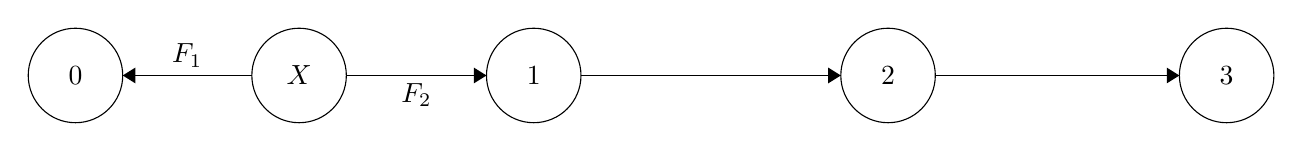
\begin{tikzpicture}[scale=0.2]
    \tikzstyle{every node}+=[inner sep=0pt]
    \draw [black] (32.4,-22.1) circle (3);
    \draw (32.4,-22.1) node {$1$};
    \draw [black] (54.9,-22.1) circle (3);
    \draw (54.9,-22.1) node {$2$};
    \draw [black] (3.3,-22.1) circle (3);
    \draw (3.3,-22.1) node {$0$};
    \draw [black] (76.4,-22.1) circle (3);
    \draw (76.4,-22.1) node {$3$};
    \draw [black] (17.5,-22.1) circle (3);
    \draw (17.5,-22.1) node {$X$};
    \draw [black] (35.4,-22.1) -- (51.9,-22.1);
    \fill [black] (51.9,-22.1) -- (51.1,-21.6) -- (51.1,-22.6);
    \draw [black] (57.9,-22.1) -- (73.4,-22.1);
    \fill [black] (73.4,-22.1) -- (72.6,-21.6) -- (72.6,-22.6);
    \draw [black] (14.5,-22.1) -- (6.3,-22.1);
    \fill [black] (6.3,-22.1) -- (7.1,-22.6) -- (7.1,-21.6);
    \draw (10.4,-21.6) node [above] {$F_{1}$};
    \draw [black] (20.5,-22.1) -- (29.4,-22.1);
    \fill [black] (29.4,-22.1) -- (28.6,-21.6) -- (28.6,-22.6);
    \draw (24.95,-22.6) node [below] {$F_{2}$};
    \end{tikzpicture}
    \end{center}
\end{figure}
Recordemos que el meteorito está en una posición válida la suma de las fuerzas debe ser igual con cero:
\[
    F_{1} + F_{2} + F_{3} + F_{3} = 0 
\]
¿Que ocurre si la suma de fuerzas no es igual con cero? Debemos de mover nuestra binaria. Si la suma es mayor que cero nos movemos a la izquierda, si es menor que cero nos movemos a la derecha.

Tomar en cuenta que si eliminas de la fórmula el valor absoluto no necesitaremos comprobar la posición del planeta en la que estamos. Si es negativo el resultado de el elemento de la fórmula que estamos haciendo entonces la fuerza que tenemos esta a la derecha en otro caso está a la izquierda.

\begin{lstlisting}
    #include <bits/stdc++.h>

    using namespace std;
    vector< double > planets;
    int n;
    //\sum^{ n }_{ 0 }{ \frac{ 1 }{ X_{i} - M } }
    double SumOfForces( double middle ){
        double sum = 0.0;
        for( int i = 0; i < n; i++ ){
            sum += 1 / ( planets[ i ] - middle );
        }
        return sum;
    }

    int main(){
        ios::sync_with_stdio( false );
        cout.tie( nullptr );
        cin.tie( nullptr );
        cin >> n;
        planets.resize( n );
        for( int i = 0; i < n; i++)
            cin >> planets[ i ];
        sort( planets.begin(), planets.end() );
        cout << n - 1 << endl; 
        for( int i = 0; i < n - 1; i++ ){
            double begin = planets[ i ];
            double end = planets[ i + 1 ];
            double middle;
            for( int i = 0; i < 25; i++ ){
                middle = ( begin + end ) / 2;
                if( SumOfForces( middle ) < 0 ){
                    begin = middle;
                } else {
                    end = middle;
                }
            }
            cout << fixed;
            cout << setprecision( 3 );
            cout << middle << " "; 
        }
        cout << endl;
        return 0;
    }
\end{lstlisting}
\chapter{Programación dinámica}
Partimos de una solución recursiva bruta y podemos hacer uso de una función de memorización. El ejemplo más clásico es el de Fibonacci
\section{Fibonacci}
\[
    fibonacci(n) = 
    \begin{cases*}
        0 & , $n = 0$ \\    
        1 & , $n = 1$ \\
        fibonacci( n - 1 ) + fibonacci( n - 2 ) & , $ n \geq 2$ 
    \end{cases*}    
\]

En código
\begin{lstlisting}
    int fibonacci( int n ){
        if( n == 0 )
            return 0;
        if( n == 1 )
            return 1;
        return fibonacci( n - 1 ) * fibonacci( n - 2 );
    }
\end{lstlisting}

Si dibujamos las llamadas recursivas como un árbol tenemos lo siguiente 

\begin{figure}[H]
    \begin{center}
        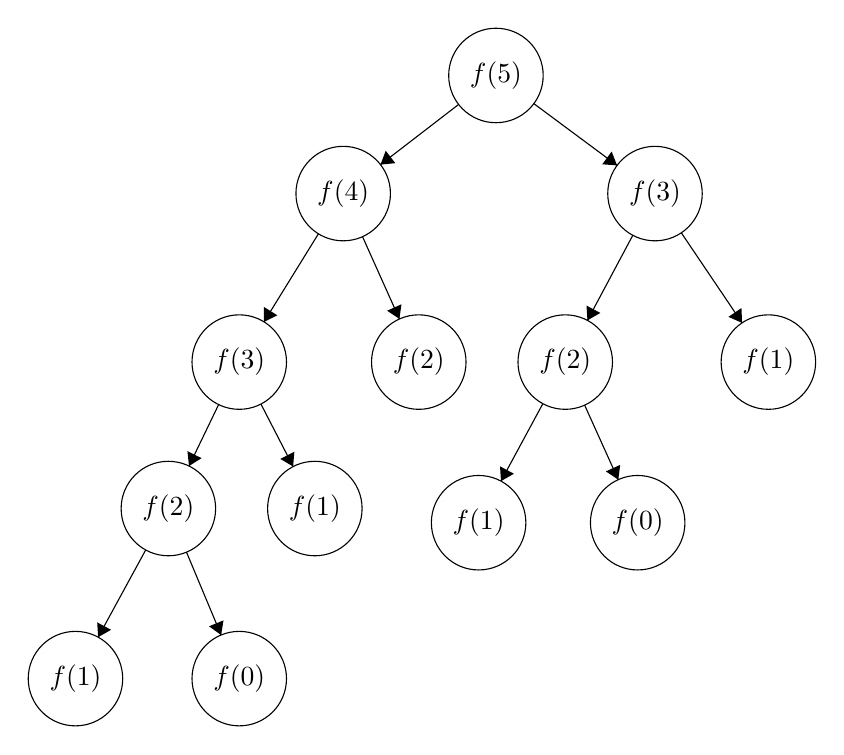
\begin{tikzpicture}[scale=0.2]
        \tikzstyle{every node}+=[inner sep=0pt]
        \draw [black] (38.5,-6.8) circle (3);
        \draw (38.5,-6.8) node {$f(5)$};
        \draw [black] (28.8,-14.3) circle (3);
        \draw (28.8,-14.3) node {$f(4)$};
        \draw [black] (48.6,-14.3) circle (3);
        \draw (48.6,-14.3) node {$f(3)$};
        \draw [black] (22.2,-25) circle (3);
        \draw (22.2,-25) node {$f(3)$};
        \draw [black] (33.6,-25) circle (3);
        \draw (33.6,-25) node {$f(2)$};
        \draw [black] (42.9,-25) circle (3);
        \draw (42.9,-25) node {$f(2)$};
        \draw [black] (55.8,-25) circle (3);
        \draw (55.8,-25) node {$f(1)$};
        \draw [black] (17.7,-34.3) circle (3);
        \draw (17.7,-34.3) node {$f(2)$};
        \draw [black] (27,-34.3) circle (3);
        \draw (27,-34.3) node {$f(1)$};
        \draw [black] (11.8,-45.1) circle (3);
        \draw (11.8,-45.1) node {$f(1)$};
        \draw [black] (22.2,-45.1) circle (3);
        \draw (22.2,-45.1) node {$f(0)$};
        \draw [black] (37.4,-35.2) circle (3);
        \draw (37.4,-35.2) node {$f(1)$};
        \draw [black] (47.5,-35.2) circle (3);
        \draw (47.5,-35.2) node {$f(0)$};
        \draw [black] (36.13,-8.64) -- (31.17,-12.46);
        \fill [black] (31.17,-12.46) -- (32.11,-12.37) -- (31.5,-11.58);
        \draw [black] (40.91,-8.59) -- (46.19,-12.51);
        \fill [black] (46.19,-12.51) -- (45.85,-11.63) -- (45.25,-12.44);
        \draw [black] (27.23,-16.85) -- (23.77,-22.45);
        \fill [black] (23.77,-22.45) -- (24.62,-22.03) -- (23.77,-21.5);
        \draw [black] (30.03,-17.04) -- (32.37,-22.26);
        \fill [black] (32.37,-22.26) -- (32.5,-21.33) -- (31.59,-21.74);
        \draw [black] (50.27,-16.79) -- (54.13,-22.51);
        \fill [black] (54.13,-22.51) -- (54.09,-21.57) -- (53.26,-22.13);
        \draw [black] (47.19,-16.95) -- (44.31,-22.35);
        \fill [black] (44.31,-22.35) -- (45.13,-21.88) -- (44.25,-21.41);
        \draw [black] (20.89,-27.7) -- (19.01,-31.6);
        \fill [black] (19.01,-31.6) -- (19.81,-31.1) -- (18.91,-30.66);
        \draw [black] (23.58,-27.67) -- (25.62,-31.63);
        \fill [black] (25.62,-31.63) -- (25.7,-30.69) -- (24.81,-31.15);
        \draw [black] (16.26,-36.93) -- (13.24,-42.47);
        \fill [black] (13.24,-42.47) -- (14.06,-42) -- (13.18,-41.53);
        \draw [black] (18.85,-37.07) -- (21.05,-42.33);
        \fill [black] (21.05,-42.33) -- (21.2,-41.4) -- (20.28,-41.78);
        \draw [black] (41.48,-27.64) -- (38.82,-32.56);
        \fill [black] (38.82,-32.56) -- (39.64,-32.09) -- (38.76,-31.62);
        \draw [black] (44.13,-27.73) -- (46.27,-32.47);
        \fill [black] (46.27,-32.47) -- (46.39,-31.53) -- (45.48,-31.94);
        \end{tikzpicture}
    \end{center}
\end{figure}

Como podemos observar hay llamadas recursivas que se repiten varias veces como ejemplo tenemos la llamada recursiva con un valor de 3, o 2. ¿Podemos evitar esto?

\begin{lstlisting}
    int memoria[ 100000 ];
    .
    .
    .
    int fibonacci( int n ){
        if( n == 0 )
            return 0;
        if( n == 1 )
            return 1;
        if( memoria[ n ] != -1 )
            return memoria[ n ];
        return memoria[ n ] = ( fibonacci( n - 1 ) * fibonacci( n - 2 ) );
    }

    int main(){
        memset( memoria, -1, sizeof(memoria) );
        .
        .
        .
    }
\end{lstlisting}

La complejidad la podemos calcular viendo los estados, en nuestro caso es el tamaño de la memoria, por ejemplo si llamamos a fibonacci de 10 siempre tenemos el mismo resultado, por tanto multiplicamos los estados por la complejidad de la función en nuestro caso es $10^{5} * constante$

\section{Coeficiente binomial}
\[
    Coef\_Bin(n, k) = 
    \begin{cases*}
        1 & , $n = k$ \\    
        1 & , $k = 0$ \\
        Coef\_Bin( n - 1, k - 1 ) + Coef\_Bin( n - 1, k ) & , $ k \leq n$ 
    \end{cases*}    
\]

Si programamos esta función tenemos lo siguiente: 

\begin{lstlisting}
    int coef_bin( int n, int k ){
        if( n == k || k == 0 )
            return 1;
        return ( coef_bin( n - 1, k - 1 ) + coef_bin( n - 1, k ) ); 
    }
\end{lstlisting}

Si aplicamos DP
\begin{lstlisting}
    memoria[ 1000 ][ 1000 ];
    .
    .
    .
    int coef_bin( int n, int k ){
        if( n == k || k == 0 )
            return 1;
        if( mem[ n ][ k ] != -1 )
            return memoria[ n ][ k ];
        return memoria[ n ][ k ] = ( coef_bin( n - 1, k - 1 ) + coef_bin( n - 1, k ) ); 
    }
\end{lstlisting}
En complejidad tenemos $O(n * k)$ y sin la función de memorización tenemos $O(2^{n})$

\section{Problema}
\textbf{Dado un grid de $n x m$, cada casilla tiene un número. Obtener un camino de la fila 1 a la fila n con suma máxima, ejemplo: }

\begin{longtable}[c]{|l|l|l|}
    \hline
    \rowcolor[HTML]{FFFFFF} 
    3                         & {\color[HTML]{333333} 5}                         & \cellcolor[HTML]{C0C0C0}{\color[HTML]{333333} 10} \\ \hline
    \endfirsthead
    %
    \endhead
    %
    \rowcolor[HTML]{FFFFFF} 
    6                         & \cellcolor[HTML]{C0C0C0}{\color[HTML]{333333} 4} & {\color[HTML]{333333} 3}                          \\ \hline
    \cellcolor[HTML]{C0C0C0}2 & 1                                                & 0                                                 \\ \hline
\end{longtable}

Como restricciones tenemos que $n, m \leq 10^{3}$ y además $A_{i,j} \leq 10^{6}$ Además solo nos podemos mover de la siguiente manera. Supongamos que estamos en el recuadro con el color gris más oscuro, estando en esa posición podemos movernos a cualquiera de los tres rectangulos con color gris más claro, es decir, podemos movernos hacía $(f + 1, c), (f + 1, c - 1), (f + 1, c + 1)$

\begin{longtable}[c]{|l|l|l|}
    \hline
    \rowcolor[HTML]{FFFFFF} 
     & \cellcolor[HTML]{656565}{\color[HTML]{333333} } & {\color[HTML]{333333} } \\ \hline
    \endfirsthead
    %
    \endhead
    %
    \rowcolor[HTML]{C0C0C0} 
     & {\color[HTML]{333333} }                         & {\color[HTML]{333333} } \\ \hline
\end{longtable}

\subsection{Solución}
\begin{lstlisting}
    int max_sum( int f, int c ){
        //Primero comprobamos si es un caso válido
        if( c < 0 || c >= m )
            return MIN_INT //MIN_INT es como un menos infinito
        //Caso base
        if( f == n )
            return grid[ f ][ c ];
        int A = max_sum( f + 1, c - 1);
        int B = max_sum( f + 1, c );
        int C = max_sum( f + 1, c + 1 );
        //No exite una función max para 3 elementos, en dado caso podemos usar vector es decir ponemos max({A, B, C})
        return max( A, max(B, C) ) + grid[ f ][ c ];
    }
\end{lstlisting}

Ahora bien ¿Cómo reducimos la complejidad de el código anterior? Debemos aplicar programación dinámica, primeramente ¿Cuál es el tamaño máximo de nuestra función de memoria? en nuestro caso es 1005 * 1005

\begin{lstlisting}
    int memoria[ 1005 ][ 1005 ];
    .
    .
    .
    int max_sum( int f, int c ){
        //Primero comprobamos si es un caso válido (que no esté fuera de rango)
        if( c < 0 || c >= m )
            return -1 //-1 es un valor bandera que identifica si ya visitamos o no la casilla
        //Caso base
        if( f == n )
            return grid[ f ][ c ];

        if( memoria[ f ][ c ] != -1 )
            return memoria[ f ][ c ]

        int A = max_sum( f + 1, c - 1);
        int B = max_sum( f + 1, c );
        int C = max_sum( f + 1, c + 1 );
        //No exite una función max para 3 elementos, en dado caso podemos usar vector es decir ponemos max({A, B, C})
        return memoria[ f ][ c ] = max( A, max(B, C) ) + grid[ f ][ c ];
    }
\end{lstlisting}

\section{Problema}
Del ejercicio anterior que sucede si podemos añadir ¿números negativos? Podemos hacer uso de otro arreglo auxiliar de booleanos, en el que marcamos si ya visitamos o no una casilla

\chapter{Problemas clásicos de DP}
\section{Mochilas}
\textbf{Vas a una tienda y quieres comprar algunos productos, digamos que hay n productos y cada producto tiene un precio y tenemos M pesos para gastar. Queremos comprar la mayor cantidad de productos gastando lo más posible.\\}
\textbf{Restricciones:}
\begin{itemize}
    \item N productos $N \leq 1000$
    \item M Pesos $M \leq 1000$
    \item $A_{i} \leq 1000$
\end{itemize}
Ejemplo:\\
N = 3, M = 8, y tenemos los productos A = {3, 4, 6} nuestro solución es comprar {3, 4} el precio es 7 y nos llevamos 4 productos.\\\\
Para poder solucionar este problema debemos de calcular el caso de probar y no probar el i-ésimo elemento. Es decir generamos todos los posibles subconjuntos del arreglo:
\begin{itemize}
    \item ()
    \item (3)
    \item (3, 4)
    \item (3, 6)
    \item (4)
    \item (4, 6)
    \item (6)
    \item (3, 4, 6)
\end{itemize}
\begin{lstlisting}
    int max_sum( int indice, int pesos_restantes ){
        //Validación, n es el número de elementos del arreglo A
        if( indice >= n )
            return 0;
        //Como no es una respuesta válida para descartarla regresamos un menos infinito
        if( pesos_restantes < 0)
            return MIN_INT;
        //Recursivamente puedo tomar o no tomar un elemento
        int tomar = max_sum( indice + 1, pesos - A[ indice ]) + A[ indice ];
        int no_tomar = max_sum( indice + 1, pesos);
        return max( tomar, no_tomar );
    }
\end{lstlisting}

Esta solución es la más bruta si queremos aplicar programación dinámica ¿Cuáles son los estados que tenemos? En este caso tendremos los índices y la cantidad de pesos restantes. Es decir:
\begin{lstlisting}
    .
    .
    .
    int memoria[ 1005 ][ 1005 ];
    bool visitado[ 1005 ][ 1005 ];
    .
    .
    .
    int max_sum( int indice, int pesos_restantes ){
        //Validación, n es el número de elementos del arreglo A
        if( indice >= n )
            return 0;
        //Como no es una respuesta válida para descartarla regresamos un menos infinito
        if( pesos_restantes < 0)
            return MIN_INT;

        if( visitado[ indice ][ pesos_restantes ] )
            return memoria[ indice ][ pesos_restantes ];
        
        //Recursivamente puedo tomar o no tomar un elemento
        int tomar = max_sum( indice + 1, pesos - A[ indice ]) + A[ indice ];
        int no_tomar = max_sum( indice + 1, pesos);
        //Como no se ha visitado el cálculo actual lo marcamos como visitado
        visitado[ indice ][ pesos_restantes ] = true;
        //Almacenamos el valor calculado en nuestra memoria
        return memoria[ indice ][ pesos_restantes ] = max( tomar, no_tomar );
    }
\end{lstlisting}

Con esta solución tenemos una complejidad de $O(n^{2})$ mientras que la solución bruta tiene una complejidad de $O(2^{n})$

\section{Mochila clásica}
\textbf{Queremos meter N piedras a una mochila cuya capacidad es de M y cada piedra tiene un valor V, queremos meter la mayor cantidad de piedras respetando que el peso límite soportado por la mochila no se exceda y se maximice el valor de las piedras dentro de la mochila\\}
\textbf{Restricciones:}
\begin{itemize}
    \item N piedras $N \leq 1000$
    \item M capacidad de la mochila $M \leq 1000$
    \item $V_{i}$ valor de la piedra $ V_{i} \leq 10^{9}$
    \item $W_{i}$ peso de la piedra $W_{i} \leq 1000$
\end{itemize}
Ejemplo:\\
N = 3, M = 50;\\
V = [ 60, 100, 120 ]\\
W = [ 10, 20, 30 ]\\
Para este caso tenemos como solución tomar la segunda y tercer piedra teniendo un valor de 220 y un peso de 50, el cual puede soportar perfectamente nuestra mochila.\\

Podemos encontrar una solución siguiendo más o menos lo mismo que el ejercico anterior, vamos a tratar de maximizar el valor tomando o no tomando el i-ésimo peso 

\begin{lstlisting}
    int sum_max( int indice, int capacidad ){
        if( indice >= n )
            return 0;
        if( capacidad < 0 )
            return MIN_INT;
        //Si lo tomo cuál es el valor máximo que podemos tener con la respuesta actual?
        int tomar = sum_max( indice + 1, capacidad - W[ indice ] ) + V[ indice ];
        int no_tomar = sum_max( indice + 1, capacidad );
        return max(tomar, no_tomar);
    }
\end{lstlisting}

Si aplicamos programación dinámica
\begin{lstlisting}
    .
    .
    .
    int memoria[ 1005 ][ 1005 ];
    .
    .
    .
    int sum_max( int indice, int capacidad ){
        if( indice >= n )
            return 0;
        if( capacidad < 0 )
            return MIN_INT;
        if( memoria[ indice ][ capacidad ] != MIN_INT )
            return memoria[ indice ][ capacidad ];
        //Si lo tomo cuál es el valor máximo que podemos tener con la respuesta actual?
        int tomar = sum_max( indice + 1, capacidad - W[ indice ] ) + V[ indice ];
        int no_tomar = sum_max( indice + 1, capacidad );
        return memoria[ indice ][ capacidad ] = max(tomar, no_tomar);
    }
\end{lstlisting}

Ahora bien debemos responder ¿dónde está la respuesta a nuestro problema?

\begin{lstlisting}
    .
    .
    .
    int main(){
        .
        .
        .
        //Si indexamos desde cero aquí estará la solución
        cout << sum_max( 0, M );
        .
        .
        .
        return 0;
    }
\end{lstlisting}

\section{Problema}
\textbf{Imagina que compraste algo en algúna tienda, supermercado, etc, tienes que pagar con N monedas, pero quieres saber ¿De cuantas formas utilizando cualquiera de esas N monedas puedo dar el cambio (M)?\\}
\textbf{Restricciones: }
\begin{itemize}
    \item N monedas $N \leq 1000$
    \item M cambio $N \leq 1000$
    \item $C_{i}$ Monedas $1 leq C_{i} \leq 1000$
\end{itemize}
Ejemplo:
N = 4, M = 5\\
C = [ 1, 2, 3, 4 ] //Indexado desde cero \\
\begin{itemize}
    \item { (0, 3) = 1 + 4 = 5 }
    \item { (1, 2) = 2 + 3 = 5 }
\end{itemize}

Es decir nuevamente debemos de considerar el problema como tomar o no tomar

\begin{figure}[H]
    
\begin{center}
    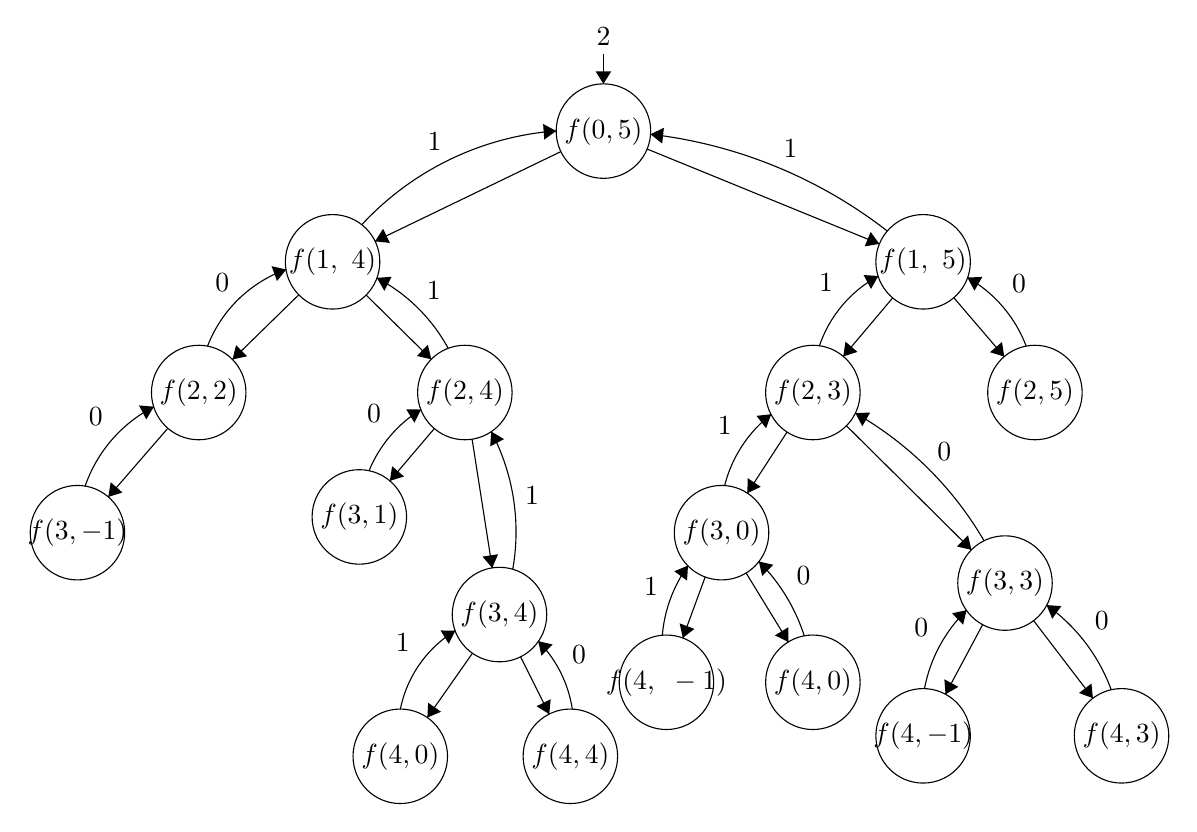
\begin{tikzpicture}[scale=0.2]
    \tikzstyle{every node}+=[inner sep=0pt]
    \draw [black] (38.5,-6.8) circle (3);
    \draw (38.5,-6.8) node {$f(0,5)$};
    \draw [black] (21.3,-15.1) circle (3);
    \draw (21.3,-15.1) node {$f(1,\mbox{ }4)$};
    \draw [black] (58.8,-15.1) circle (3);
    \draw (58.8,-15.1) node {$f(1,\mbox{ }5)$};
    \draw [black] (12.8,-23.4) circle (3);
    \draw (12.8,-23.4) node {$f(2,2)$};
    \draw [black] (29.7,-23.4) circle (3);
    \draw (29.7,-23.4) node {$f(2,4)$};
    \draw [black] (5.1,-32.3) circle (3);
    \draw (5.1,-32.3) node {$f(3,-1)$};
    \draw [black] (51.8,-23.4) circle (3);
    \draw (51.8,-23.4) node {$f(2,3)$};
    \draw [black] (65.9,-23.4) circle (3);
    \draw (65.9,-23.4) node {$f(2,5)$};
    \draw [black] (23,-31.3) circle (3);
    \draw (23,-31.3) node {$f(3,1)$};
    \draw [black] (31.9,-37.5) circle (3);
    \draw (31.9,-37.5) node {$f(3,4)$};
    \draw [black] (25.6,-46.5) circle (3);
    \draw (25.6,-46.5) node {$f(4,0)$};
    \draw [black] (36.4,-46.5) circle (3);
    \draw (36.4,-46.5) node {$f(4,4)$};
    \draw [black] (46,-32.3) circle (3);
    \draw (46,-32.3) node {$f(3,0)$};
    \draw [black] (64,-35.5) circle (3);
    \draw (64,-35.5) node {$f(3,3)$};
    \draw [black] (58.8,-45.2) circle (3);
    \draw (58.8,-45.2) node {$f(4,-1)$};
    \draw [black] (71.4,-45.2) circle (3);
    \draw (71.4,-45.2) node {$f(4,3)$};
    \draw [black] (42.5,-41.8) circle (3);
    \draw (42.5,-41.8) node {$f(4,\mbox{ }-1)$};
    \draw [black] (51.8,-41.8) circle (3);
    \draw (51.8,-41.8) node {$f(4,0)$};
    \draw [black] (35.8,-8.1) -- (24,-13.8);
    \fill [black] (24,-13.8) -- (24.94,-13.9) -- (24.51,-13);
    \draw [black] (41.28,-7.94) -- (56.02,-13.96);
    \fill [black] (56.02,-13.96) -- (55.47,-13.2) -- (55.09,-14.12);
    \draw [black] (19.15,-17.2) -- (14.95,-21.3);
    \fill [black] (14.95,-21.3) -- (15.87,-21.1) -- (15.17,-20.39);
    \draw [black] (23.43,-17.21) -- (27.57,-21.29);
    \fill [black] (27.57,-21.29) -- (27.35,-20.37) -- (26.65,-21.08);
    \draw [black] (10.84,-25.67) -- (7.06,-30.03);
    \fill [black] (7.06,-30.03) -- (7.96,-29.75) -- (7.21,-29.1);
    \draw [black] (56.87,-17.39) -- (53.73,-21.11);
    \fill [black] (53.73,-21.11) -- (54.63,-20.82) -- (53.87,-20.17);
    \draw [black] (60.75,-17.38) -- (63.95,-21.12);
    \fill [black] (63.95,-21.12) -- (63.81,-20.19) -- (63.05,-20.84);
    \draw [black] (27.76,-25.69) -- (24.94,-29.01);
    \fill [black] (24.94,-29.01) -- (25.84,-28.73) -- (25.08,-28.08);
    \draw [black] (30.16,-26.36) -- (31.44,-34.54);
    \fill [black] (31.44,-34.54) -- (31.81,-33.67) -- (30.82,-33.82);
    \draw [black] (30.18,-39.96) -- (27.32,-44.04);
    \fill [black] (27.32,-44.04) -- (28.19,-43.67) -- (27.37,-43.1);
    \draw [black] (33.24,-40.18) -- (35.06,-43.82);
    \fill [black] (35.06,-43.82) -- (35.15,-42.88) -- (34.25,-43.32);
    \draw [black] (50.16,-25.91) -- (47.64,-29.79);
    \fill [black] (47.64,-29.79) -- (48.49,-29.39) -- (47.66,-28.84);
    \draw [black] (53.93,-25.51) -- (61.87,-33.39);
    \fill [black] (61.87,-33.39) -- (61.65,-32.47) -- (60.95,-33.18);
    \draw [black] (62.58,-38.14) -- (60.22,-42.56);
    \fill [black] (60.22,-42.56) -- (61.04,-42.09) -- (60.15,-41.61);
    \draw [black] (65.82,-37.89) -- (69.58,-42.81);
    \fill [black] (69.58,-42.81) -- (69.49,-41.88) -- (68.7,-42.48);
    \draw [black] (23.154,-12.745) arc (137.20989:94.31013:18.749);
    \fill [black] (35.5,-6.79) -- (34.67,-6.35) -- (34.74,-7.34);
    \draw (27.78,-8.09) node [above] {$1$};
    \draw [black] (13.355,-20.468) arc (159.00785:109.62803:8.366);
    \fill [black] (18.36,-15.59) -- (17.43,-15.38) -- (17.77,-16.32);
    \draw (14.3,-17) node [above] {$0$};
    \draw [black] (5.585,-29.354) arc (-198.95042:-242.78023:8.946);
    \fill [black] (9.95,-24.3) -- (9.01,-24.22) -- (9.47,-25.11);
    \draw (6.74,-24.96) node [left] {$0$};
    \draw [black] (24.111,-16.121) arc (62.21244:28.47373:10.983);
    \fill [black] (24.11,-16.12) -- (24.59,-16.94) -- (25.05,-16.05);
    \draw (27.73,-17.55) node [above] {$1$};
    \draw [black] (23.611,-28.38) arc (157.76368:121.63368:8.246);
    \fill [black] (26.92,-24.48) -- (25.98,-24.47) -- (26.5,-25.32);
    \draw (24.41,-24.72) node [left] {$0$};
    \draw [black] (31.377,-25.88) arc (27.76697:-10.03044:13.665);
    \fill [black] (31.38,-25.88) -- (31.31,-26.82) -- (32.19,-26.36);
    \draw (33.49,-29.94) node [right] {$1$};
    \draw [black] (25.601,-43.519) arc (-191.3248:-238.65924:7.6);
    \fill [black] (29.1,-38.52) -- (28.16,-38.51) -- (28.68,-39.36);
    \draw (26.23,-39.29) node [left] {$1$};
    \draw [black] (34.359,-39.186) arc (44.59265:8.53745:7.831);
    \fill [black] (34.36,-39.19) -- (34.56,-40.11) -- (35.28,-39.4);
    \draw (36.48,-40.07) node [right] {$0$};
    \draw [black] (46.194,-29.323) arc (-194.05678:-232.12662:8.313);
    \fill [black] (49.15,-24.78) -- (48.22,-24.88) -- (48.83,-25.67);
    \draw (46.68,-25.48) node [left] {$1$};
    \draw [black] (52.21,-20.446) arc (-198.71388:-241.57291:7.955);
    \fill [black] (55.96,-16) -- (55.02,-15.94) -- (55.49,-16.82);
    \draw (53.11,-16.43) node [left] {$1$};
    \draw [black] (61.613,-16.096) arc (60.36187:20.72692:8.481);
    \fill [black] (61.61,-16.1) -- (62.06,-16.93) -- (62.56,-16.06);
    \draw (64.41,-16.51) node [right] {$0$};
    \draw [black] (54.497,-24.708) arc (60.25935:30.21222:22.202);
    \fill [black] (54.5,-24.71) -- (54.94,-25.54) -- (55.44,-24.67);
    \draw (60.14,-27.74) node [above] {$0$};
    \draw [black] (58.883,-42.214) arc (-190.71414:-225.67582:9.427);
    \fill [black] (61.56,-37.22) -- (60.64,-37.42) -- (61.34,-38.14);
    \draw (59.16,-38.34) node [left] {$0$};
    \draw [black] (66.643,-36.902) arc (54.54567:20.13338:11.436);
    \fill [black] (66.64,-36.9) -- (67,-37.77) -- (67.58,-36.96);
    \draw (69.67,-37.88) node [right] {$0$};
    \draw [black] (41.492,-6.999) arc (83.35606:52.16787:30.209);
    \fill [black] (41.49,-7) -- (42.23,-7.59) -- (42.34,-6.59);
    \draw (50.39,-8.53) node [above] {$1$};
    \draw [black] (44.96,-35.12) -- (43.54,-38.98);
    \fill [black] (43.54,-38.98) -- (44.28,-38.41) -- (43.34,-38.06);
    \draw [black] (47.56,-34.86) -- (50.24,-39.24);
    \fill [black] (50.24,-39.24) -- (50.25,-38.3) -- (49.39,-38.82);
    \draw [black] (42.239,-38.826) arc (-184.72078:-215.72893:8.834);
    \fill [black] (43.87,-34.39) -- (43,-34.75) -- (43.81,-35.34);
    \draw (42,-35.7) node [left] {$1$};
    \draw [black] (48.368,-34.129) arc (45.01101:17.79931:11.777);
    \fill [black] (48.37,-34.13) -- (48.58,-35.05) -- (49.29,-34.34);
    \draw (50.73,-35.05) node [right] {$0$};
    \draw [black] (38.5,-1.9) -- (38.5,-3.8);
    \draw (38.5,-1.4) node [above] {$2$};
    \fill [black] (38.5,-3.8) -- (39,-3) -- (38,-3);
    \end{tikzpicture}
    \end{center}
\end{figure}

Como solución bruta ¿Qué podemos programar?
\begin{lstlisting}
    .
    .
    .
    int cuenta( int indice, int cambio ){
        //Verificamos que no nos salgamos del rango
        if( indice == n ){
            //Si llegamos al límite verificamos si lo que tenemos es una solución válida
            if( cambio == 0 )
                //Como encontramos una solución la contamos
                return 1;
            //Como no hay solución retornamos cero
            return 0;
        }
        //Si el cambio es negativo no es una combinación válida
        if( cambio < 0 )
            return 0;
        //Intentamos tomando el elemento actual
        int tomar = cuenta( indice + 1, cambio - C[ indice ] );
        int no_tomar = cuenta( indice + 1, cambio );
        return tomar + no_tomar;
    }
\end{lstlisting}

Si añadimos programación dinámica tenemos lo siguiente

\begin{lstlisting}
    .
    .
    .
    int memoria[ 1005 ][ 1005 ];
    bool visitado[ 1005 ][ 1005 ];
    .
    .
    .
    int cuenta( int indice, int cambio ){
        //Verificamos que no nos salgamos del rango
        if( indice == n ){
            //Si llegamos al límite verificamos si lo que tenemos es una solución válida
            if( cambio == 0 )
                //Como encontramos una solución la contamos
                return 1;
            //Como no hay solución retornamos cero
            return 0;
        }
        //Si el cambio es negativo no es una combinación válida
        if( cambio < 0 )
            return 0;
    
        if( visitado[ indice ][ cambio ] )
            return memoria[ indice ][ cambio ];
        //Intentamos tomando el elemento actual
        int tomar = cuenta( indice + 1, cambio - C[ indice ] );
        int no_tomar = cuenta( indice + 1, cambio );
        visitado[ indice ][ cambio ] = true;
        return memoria[ indice ][ cambio ] = (tomar + no_tomar);
    }
\end{lstlisting}


\section{Boredrom}
\textbf{Vamos a tomar el $a_{k}$ elemento, vamos remover de nuestro arrego el $a_{k} + 1$ y $a_{k} - 1$ }\\
\textbf{Restricciones: }
1 1 2 2 2 2 2 3 3 \\
En este caso elegimos el 2 y removemos los unos y los tres nos queda \\
2 2 2 2 2 \\ 
Como no tenemos más elementos para elegir nuestra respuesta es la suma de los elementos restantes es decir 5 \\
¿Cómo podemos programar eso?
\begin{lstlisting}
    #include <bits/stdc++.h>

    using namespace std;
    typedef long long int lli;
    lli bucket[ 100005 ];
    lli DP[ 100005 ];
    bool visited[ 100005 ];
    lli n;
    int MAX = -1;
    
    lli max_sum( int index ){
    
        if( index >= MAX + 1)
            return 0;
        
        if( visited[ index ] )
            return DP[ index ];
        visited[ index ] = true;
        //Tomamos el elemento actual
        lli take = max_sum( index + 2 ) + ( bucket[ index ] * index );
        //Nos saltamos el elemento actual
        lli not_take = max_sum( index + 1 );
    
        return DP[ index ] = max( take, not_take );
    }
    
    int main(){
        cin >> n;
        for( int i = 0, v; i < n; i++){
            cin >> v;
            MAX = max( MAX, v );
            //Generamos nuestra cubeta
            bucket[ v ]++;
        }
        
        cout << max_sum( 1 ) << endl;
        return 0;
    }
\end{lstlisting}

\section{LIS - Longest Increasing Subsequence}
Nos sirve para encontrar la subsecuencia más larga que sea creciente. Por ejemplo:\\\\

[1, 5, 3, 7, 8, 4]\\\\

Tenemos algunas posibilidades\\\\

5, 7, 4 consideremos que el conjunto vacío también es válido. Pero esta subsecuencia no es creciente.\\\\ 

Pero si las siguientes 1, 5, 7, 8 y 1, 3, 7, 8. dónde la resuesta es 4.\\\\

¿Cómo podemos solucionar esto? Podemos calcular todos los pusibles subconjuntos haciendo algo similar al problema de la mochila, es decir, tomar o no tomar. También requerimos conocer el número anterior ya que este nos ayudará a decidir si el número actual podemos tomarlo o no.
\textbf{Restricciones: }
\begin{itemize}
    \item $0 < n \leq 1000$
    \item $0 < A_{i} \leq 1000$
\end{itemize}
\begin{lstlisting}
    int LIS( int index, int last ){
        //Caso base 
        if( indice == n )
            return 0;
        
        //Vamos a tomar como válido el valor si y solo si si el i-ésimo elemento es mayor que el i-ésimo - 1
        if( A[ index ] > last ){
            int take = LIS( index + 1, A[ index ] ) + 1;
            int not_take = LIS( index + 1, last );
            return max( take, not_take );
        }
        return LIS( index + 1, last );
    }
    .
    .
    .
    int main(){
        .
        .
        .
            cout << LIS( 0, INT_MIN ) << endl;
        .
        .
        .
    }
\end{lstlisting}

Esta solución obtiene todos los subconjuntos pero la complejidad es de $O(2^{n})$. Si queremos optimizar usando memoria debemos ver los estados de nuestra DP, en este caso tenemos dos, el primero el índice y el segundo el valor más grande que puede valer last, es decir, 1000 y 1000 respectivamente. Por tanto obtenemos cono resultado

\begin{lstlisting}
    .
    .
    .
    int DP[ 1005 ][ 1005 ] = { -1 };
    .
    .
    .
    int LIS( int index, int last ){
        //Caso base 
        if( indice == n )
            return 0;
        if( DP[ index ][ last ] != -1 )
            return DP[ index ][ last ];
        //Vamos a tomar como válido el valor si y solo si si el i-ésimo elemento es mayor que el i-ésimo - 1
        if( A[ index ] > last ){
            int take = LIS( index + 1, A[ index ] ) + 1;
            int not_take = LIS( index + 1, last );
            return DP[ index ][ last ] = max( take, not_take );
        }
        return DP[ index ][ last ] = LIS( index + 1, last );
    }
    .
    .
    .
    int main(){
        .
        .
        .
            cout << LIS( 0, INT_MIN ) << endl;
        .
        .
        .
    }
\end{lstlisting}

Con esta solución la complejidad que obtenemos es de $O(n * max(A_{i}))$

Gráficamente tenemos algo como esto.

\begin{figure}[H]
    \begin{center}
    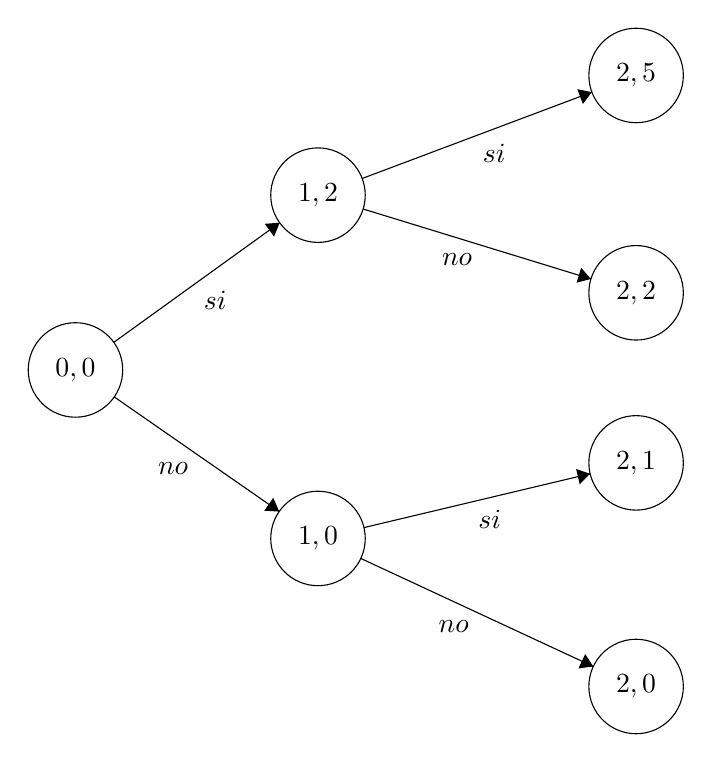
\begin{tikzpicture}[scale=0.2]
    \tikzstyle{every node}+=[inner sep=0pt]
    \draw [black] (18.7,-29.2) circle (3);
    \draw (18.7,-29.2) node {$0,0$};
    \draw [black] (34.1,-18.1) circle (3);
    \draw (34.1,-18.1) node {$1,2$};
    \draw [black] (34.1,-39.9) circle (3);
    \draw (34.1,-39.9) node {$1,0$};
    \draw [black] (54.3,-10.5) circle (3);
    \draw (54.3,-10.5) node {$2,5$};
    \draw [black] (54.3,-24.3) circle (3);
    \draw (54.3,-24.3) node {$2,2$};
    \draw [black] (54.3,-35.1) circle (3);
    \draw (54.3,-35.1) node {$2,1$};
    \draw [black] (54.3,-49.3) circle (3);
    \draw (54.3,-49.3) node {$2,0$};
    \draw [black] (21.13,-27.45) -- (31.67,-19.85);
    \fill [black] (31.67,-19.85) -- (30.72,-19.92) -- (31.31,-20.73);
    \draw (27.57,-24.15) node [below] {$si$};
    \draw [black] (21.16,-30.91) -- (31.64,-38.19);
    \fill [black] (31.64,-38.19) -- (31.26,-37.32) -- (30.69,-38.14);
    \draw (24.9,-35.05) node [below] {$no$};
    \draw [black] (36.91,-17.04) -- (51.49,-11.56);
    \fill [black] (51.49,-11.56) -- (50.57,-11.37) -- (50.92,-12.31);
    \draw (45.29,-14.83) node [below] {$si$};
    \draw [black] (36.97,-18.98) -- (51.43,-23.42);
    \fill [black] (51.43,-23.42) -- (50.81,-22.71) -- (50.52,-23.66);
    \draw (42.93,-21.77) node [below] {$no$};
    \draw [black] (37.02,-39.21) -- (51.38,-35.79);
    \fill [black] (51.38,-35.79) -- (50.49,-35.49) -- (50.72,-36.46);
    \draw (45,-38.09) node [below] {$si$};
    \draw [black] (36.82,-41.17) -- (51.58,-48.03);
    \fill [black] (51.58,-48.03) -- (51.07,-47.24) -- (50.64,-48.15);
    \draw (42.72,-45.11) node [below] {$no$};
    \end{tikzpicture}
    \end{center}
\end{figure}

Si queremos imprimir la secuencia que tenemos ¿Que podemos hacer? Podríamos usar un string o vector o también recorrer la memoria ¿Hay alguna otra solución?

Podemos reutilizar nuestra función LIS, para reconstruir la solución. Dónde vamos a añadir el valor que nos convino más como solución a nuestra respuesta. Es decir podemos tener un vector de enteros que obtenga la reconstrucción.

\begin{lstlisting}
    .
    .
    .
    vector< int > reaconstruct;
    void reconstructLIS( int index, int last ){

        if( index >= n )
            return;
        
        if( A[index] > last ){
            //Como ya se han memorizado los valores de todos los subconjuntos válidos obtendremos en constante cual camino me es más conveniente tomar
            int take = LIS( index + 1, A[ index ]) + 1;
            int not_take = LIS( index + 1, last );
            //Aquí podemos decidir que camino nos conviene más si el de tomar o no tomar
            if( take > not_take ) {
                //Añadimos a nuestra respuesta
                reconstruct.push_back( A[ index ] );
                reconstructLIS( index + 1, A[ index ] );
            } else 
                reconstructLIS( index + 1, last );
        }
        reconstructLIS( index + 1, last );
    }
    .
    .
    .
\end{lstlisting}

¿Qué complejidad tiene reconstruir la respuesta? $O( n )$ ya que solamente vamos ha realizar una sola llamada recursiva

\section{Longest Common Subsequence}
Dadas dos cadenas, hallar la subsecuencia común más larga. \\\\
\textbf{Restricciones:\\}

\textbf{Ejemplo:\\}
\begin{itemize}
    \item {S = AGPGTAB}
    \item {T = GXTXAYB}
\end{itemize}

\begin{longtable}[c]{|
    >{\columncolor[HTML]{FFFFFF}}l |
    >{\columncolor[HTML]{FFFFFF}}l |
    >{\columncolor[HTML]{FFFFFF}}l |
    >{\columncolor[HTML]{EFEFEF}}l |
    >{\columncolor[HTML]{EFEFEF}}l |
    >{\columncolor[HTML]{EFEFEF}}l |
    >{\columncolor[HTML]{EFEFEF}}l |}
    \hline
    {\color[HTML]{333333} A}                         & {\color[HTML]{333333} G} & {\color[HTML]{333333} P}                         & G                         & T                        & A                         & B                        \\ \hline
    \endfirsthead
    %
    \endhead
    %
    \cellcolor[HTML]{EFEFEF}{\color[HTML]{333333} G} & X                        & \cellcolor[HTML]{EFEFEF}{\color[HTML]{333333} T} & \cellcolor[HTML]{FFFFFF}X & {\color[HTML]{333333} A} & \cellcolor[HTML]{FFFFFF}Y & {\color[HTML]{333333} B} \\ \hline
\end{longtable}

¿Podemos atacar este problema utilizando la misma lógica que en knapsack? Si intentamos hacer esto tendremos varios problemas. Podemos remover un caracter de alguna de las dos cadenas en algún punto en el que la cadena no coincida. Si ámbos caracteres coinciden ambos los ''quitamos'' y aumentamos en 1 la respuesta actual.

\begin{lstlisting}
    int LCS( string S, string T ){

        if( S.empty() || T.empty() )
            return 0;

        string S2 = S;
        string T2 = T;
        //erase elimina el caracter (es un iterador) en nuestro caso el primero de la cadena S2
        S2.erase( S2.begin() );
        T2.erase( T2.begin() );

        //Si ámbos coinciden aumentamos en uno la respuesta
        if( S[ 0 ] == T[ 0 ] )
            //Como el caracter es el mismo en ámbos la respuesta aumenta en uno
            return LCA( S2, T2 ) + 1;

        int delete_first = LCS( S2, T );
        int delete_second = LCS( S, T2 );

        return max( delete_first, delete_second );
    }
\end{lstlisting}

¿Como podemos asegurar que nos conviene realizar lo anterior? o bien ¿Hay algún caso que no se ha cubierto? y ¿Cuál es la complejidad de este algoritmo? \\ \\

Supongamos que tenemos una cadena donde un caracter de la respuesta aparece más de una vez, si consideramos el segundo y no el primero es posible que nuestra respuesta o no mejore o empeore. \\\\

La complejidad de realizar esto es $O(2^{n} * n)$ (El n esta ahí por la función erase). ¿Cómo podemos mejorar esta solución?\\\\

Nótese que solo estamos utilizando lo caracteres del final, es decir solo utilizamos el sufijo (caracteres del final), así pues en lugar de utilizar una subcadena podemos utilizar un apuntador.

\begin{lstlisting}
    int LCS( int index_s, int index_t ){
        //Si ya no hay caracteres que analizar terminamos las recursiones
        if( index_s == S.size() || index_t == S.size() )
            return 0;
        
        if( S[index_s] == T[index_t] )
            return LCA( index_s + 1, index_t + 1) + 1;
        
        int move_S = LCS( index_s + 1, index_t );
        int move_T = LCS( index_s, index_t + 1 );

        return max( move_S, move_T );
    }
\end{lstlisting}

¿Ahora que complejidad obtenemos? $O(2^{n})$ ya que hemos eliminado el uso de la función erase. Finalmente ¿Como implementamos programación dinámica? En este caso tenemos dos estados index\_s e index\_t.

\begin{lstlisting}
    .
    .
    .
    int DP[ 1005 ][ 1005 ];
    .
    .
    .
    int LCS( int index_s, int index_t ){
        //Si ya no hay caracteres que analizar terminamos las recursiones
        if( index_s == S.size() || index_t == S.size() )
            return 0;
        //Nuestra ''bandera'' es el valor de -1 ya que nunca nos devolverá ese valor la función
        if( DP[ index_s ][ index_t ] != -1 )
            return DP[ index_s ][ index_t ]
        
        if( S[index_s] == T[index_t] )
            return DP[ index_s ][ index_t ] = LCA( index_s + 1, index_t + 1) + 1;
        
        int move_S = LCS( index_s + 1, index_t );
        int move_T = LCS( index_s, index_t + 1 );

        return DP[ index_s ][ index_t ] = max( move_S, move_T );
    }
    .
    .
    .
    int main(){
        .
        .
        .
        cout << LCS( 0, 0 ) << endl;
        .
        .
        .
        return 0;
    }
\end{lstlisting}

Y finalmente hemos optimizado sustancialmente ese problema, hemos pasado de tener una complejidad de $O(2^{n} * n)$ a $O(2^{n})$ a finalmente $O(|S|*|T|)$ o bien en $O(n^{2})$

\chapter{DP con máscaras de bits}
\section{Manipulación de bits}

Para estar en sintonía en un número binario debemos mencionar lo siguiente 
\begin{longtable}[c]{
    >{\columncolor[HTML]{FFFFFF}}l 
    >{\columncolor[HTML]{FFFFFF}}l 
    >{\columncolor[HTML]{FFFFFF}}l 
    >{\columncolor[HTML]{FFFFFF}}l 
    >{\columncolor[HTML]{FFFFFF}}l }
    \hline
    \multicolumn{1}{|l|}{\cellcolor[HTML]{FFFFFF}31}                       & \multicolumn{1}{l|}{\cellcolor[HTML]{FFFFFF}30}                       & \multicolumn{1}{l|}{\cellcolor[HTML]{FFFFFF}...}                        & \multicolumn{1}{l|}{\cellcolor[HTML]{FFFFFF}1} & \multicolumn{1}{l|}{\cellcolor[HTML]{FFFFFF}0}        \\ \hline
    \endfirsthead
    %
    \endhead
    %
    \multicolumn{1}{|l|}{\cellcolor[HTML]{FFFFFF}{\color[HTML]{333333} 0}} & \multicolumn{1}{l|}{\cellcolor[HTML]{FFFFFF}{\color[HTML]{333333} 0}} & \multicolumn{1}{l|}{\cellcolor[HTML]{FFFFFF}{\color[HTML]{333333} ...}} & \multicolumn{1}{l|}{\cellcolor[HTML]{FFFFFF}0} & \multicolumn{1}{l|}{\cellcolor[HTML]{FFFFFF}0\_\{2\}} \\ \hline
    MSB                                                                    &                                                                       &                                                                         &                                                & LSB                                                  
\end{longtable}

También tenemos varias operaciones en binario por ejemplo el AND
\begin{longtable}[c]{lllll}
    \rowcolor[HTML]{FFFFFF} 
                              & 1                        & 1                        & 0 & 0 \\
    \endfirsthead
    %
    \endhead
    %
    \rowcolor[HTML]{FFFFFF} 
    {\color[HTML]{333333} \&} & {\color[HTML]{333333} 1} & {\color[HTML]{333333} 0} & 1 & 0 \\
    \rowcolor[HTML]{C0C0C0} 
                              & 1                        & 0                        & 0 & 0
\end{longtable}

Otra operación es OR 

\begin{longtable}[c]{lllll}
    \rowcolor[HTML]{FFFFFF} 
                             & 1                        & 1                        & 0 & 0 \\
    \endfirsthead
    %
    \endhead
    %
    \rowcolor[HTML]{FFFFFF} 
    {\color[HTML]{333333} |} & {\color[HTML]{333333} 1} & {\color[HTML]{333333} 0} & 1 & 0 \\
    \rowcolor[HTML]{C0C0C0} 
                             & 1                        & 1                        & 1 & 0
\end{longtable}

Otra operación es la XOR 
\begin{longtable}[c]{lllll}
    \rowcolor[HTML]{FFFFFF} 
                                              & 1                        & 1                        & 0 & 0 \\
    \endfirsthead
    %
    \endhead
    %
    \rowcolor[HTML]{FFFFFF} 
    {\color[HTML]{333333} \textasciicircum{}} & {\color[HTML]{333333} 1} & {\color[HTML]{333333} 0} & 1 & 0 \\
    \rowcolor[HTML]{C0C0C0} 
                                              & 0                        & 1                        & 1 & 0
\end{longtable}

Negación 

\begin{longtable}[c]{lllll}
    \rowcolor[HTML]{FFFFFF} 
    $\sim$                  & 1                        & 1                        & 0 & 0 \\
    \endfirsthead
    %
    \endhead
    %
    \rowcolor[HTML]{C0C0C0} 
    {\color[HTML]{333333} } & {\color[HTML]{333333} 0} & {\color[HTML]{333333} 0} & 1 & 1
\end{longtable}

Y también tenemos optras operaciones útiles como los corrimientos de bits a la derecha o a la izquierda por ejemplo

\begin{longtable}[c]{lllll}
    \rowcolor[HTML]{FFFFFF} 
    5                        & \textless{}\textless{}                              & 2                        & = & 00...010100                    \\
    \endfirsthead
    %
    \endhead
    %
    \rowcolor[HTML]{FFFFFF} 
    {\color[HTML]{333333} 5} & {\color[HTML]{333333} \textgreater{}\textgreater{}} & {\color[HTML]{333333} 2} & = & 00...0001                      \\
    5                        & \textgreater{}\textgreater{}                        & 3+2                      & = & 5\textgreater{}\textgreater{}5
\end{longtable}

Algunas operaciones que podemos hacer por ejemplo: \newline 

Saber si el k-ésimo bit está encendido 
\begin{lstlisting}
    isSet( n, k ) bool ( n & ( 1 << k ) );
\end{lstlisting}

Colocar un uno en la k-ésima posición
\begin{lstlisting}
    setBit( n, k ) bool ( n | ( 1 << k ) );
\end{lstlisting}

Apagar el k-ésimo bit
\begin{lstlisting}
    clearBit( n, k ) bool ( n &~ ( 1 << k ) );
\end{lstlisting}

Cambiar el valor del k-ésimo bit (si es cero se vuelve uno y viceversa)

Saber si el k-ésimo bit está encendido 
\begin{lstlisting}
    isSet( n, k ) bool ( n ^ ( 1 << k ) );
\end{lstlisting}

Si queremos saber en constante el bit menos significativo de un número 

\begin{longtable}[c]{llllllll}
    \cellcolor[HTML]{FFFFFF}8                              & \cellcolor[HTML]{FFFFFF}=                        & \cellcolor[HTML]{FFFFFF}0                        & \cellcolor[HTML]{FFFFFF}... & \cellcolor[HTML]{FFFFFF}1 & 0 & 0 & 0 \\
    \endfirsthead
    %
    \endhead
    %
    \cellcolor[HTML]{FFFFFF}{\color[HTML]{333333} $\sim$8} & \cellcolor[HTML]{FFFFFF}{\color[HTML]{333333} =} & \cellcolor[HTML]{FFFFFF}{\color[HTML]{333333} 1} & \cellcolor[HTML]{FFFFFF}... & \cellcolor[HTML]{FFFFFF}0 & 1 & 1 & 1 \\
    -8                                                     & =                                                & 1                                                & ...                         & 1                         & 0 & 0 & 0 \\
    8\&-8                                                  & =                                                & 0                                                & ...                         & 1                         & 0 & 0 & 0
\end{longtable}

Por tanto obtenemos en código 
\begin{lstlisting}
    lowestBit( n, k ) (b &- n)
\end{lstlisting}


Si queremos encender los primeros K-bits pordemos hacer $2^{k} - 1$ pero ¿Podemos hacerlo más rápido? \break 

\begin{lstlisting}
    setFirstK( k ) ( ( 1 << k ) - 1);
\end{lstlisting}

¿Cómo contar el número de bits encendidos rápido? Podemos utilizar un ciclo y contar los bits ¿Pero hay una forma más fácil? \break 
en C++ tenemos una función llamada \textsf{\_\_builtin\_popcount( n )} si queremos trabajar con \textsf{long long int} podemos utilizar \textsf{\_\_builtin\_popcountll( n )}

\section{Máscaras de bits}
Tenemos lo siguiente

Los elementos que tienen un bit encendido pertenecen a un conjunto.

Si el conjunto es el vacío es pues es el que cuyo valor es cero, es decir: \newline 
$\emptyset = 0$ \newline

k elementos \newline 
$U=2^{k} - 1$ \newline

Como estamos trabajando con conjuntos ¿Que operación es la unión de dos conjuntos A y B? \newline 
$A | B$ \newline

¿La intersección de A y B? \newline
$A \& B$ \newline

El complemento \newline 
~A $\&$ U, A $\wedge$ U\newline

Insertar K en A \newline
setBit(A, k); \newline 

Eliminar K de A: \newline 
clearBit( A, k ); \newline 

\begin{itemize}
    \item { $\{\emptyset$\} }
    \item { $\{0\}$ }
    \item { $\{0, 1\}$ }
    \item { $\{0, 1, 2\}$ }
    \item { $\{0, 2\}$ }
    \item { $\{1\}$ }
    \item { $\{1, 2\}$ }
    \item { $\{2\}$ }
\end{itemize}

¿Como itero sobre todos los subconjuntos?
\begin{lstlisting}
    for( i = 0 ... i << k - 1 )
        for( j = 0 ... k - 1 )
            if( isSet(i, j) )
\end{lstlisting}

¿Cuál es la complejidad de lo anterior? $O(2^{k} * k)$

\section{Ejercicio}
Nos dan máscaras de bits, llamémosle A queremos todos los subconjuntos que hay en A por ejemplo:

\begin{longtable}[c]{|
    >{\columncolor[HTML]{FFFFFF}}l |
    >{\columncolor[HTML]{FFFFFF}}l |
    >{\columncolor[HTML]{FFFFFF}}l |
    >{\columncolor[HTML]{FFFFFF}}l |
    >{\columncolor[HTML]{FFFFFF}}l |
    >{\columncolor[HTML]{FFFFFF}}l |
    >{\columncolor[HTML]{FFFFFF}}l |
    >{\columncolor[HTML]{FFFFFF}}l |}
    \hline
    31                       &                          &                            &   &   &   &   & 0 \\ \hline
    \endfirsthead
    %
    \endhead
    %
    {\color[HTML]{333333} 0} & {\color[HTML]{333333} 0} & {\color[HTML]{333333} ...} & 1 & 1 & 0 & 1 & 0 \\ \hline
                             &                          &                            & 1 & 1 & 0 & 1 & 0 \\ \hline
                             &                          &                            & 0 & 1 & 0 & 1 & 0 \\ \hline
                             &                          &                            & 0 & 0 & 0 & 1 & 0 \\ \hline
                             &                          &                            & 1 & 0 & 0 & 0 & 0 \\ \hline
                             &                          &                            & 1 & 0 & 0 & 1 & 0 \\ \hline
                             &                          &                            & 0 & 0 & 0 & 0 & 0 \\ \hline
                             &                          &                            & 1 & 1 & 0 & 0 & 0 \\ \hline
                             &                          &                            & 0 & 1 & 0 & 0 & 0 \\ \hline
\end{longtable}



\chapter{Upsolving RPC}

\section{I. Überwatch}
Podemos utilizar DP el problema se resume en tomar y no tomar como el problema de la mochila.

\section{D. Pants on Fire}
Se quiere verificar si lo que dice un períodico es verdadero, falso o me falta información para que sea verdad. 
En el siguiente ejemplo es evidente que los Rusos son Peóres que los Mexicanos pero podemos ver que los Mexicanos son peóres que los Americanos lo podemos representar así: \break 
Rusos > Mexicanos > Americanos por tanto los Rusos son peores que los americanos (transitividad)

\begin{longtable}[c]{|
    >{\columncolor[HTML]{FFFFFF}}l |
    >{\columncolor[HTML]{FFFFFF}}l |
    >{\columncolor[HTML]{FFFFFF}}l |
    >{\columncolor[HTML]{FFFFFF}}l |
    >{\columncolor[HTML]{FFFFFF}}l |}
    \hline
    \multicolumn{5}{|l|}{\cellcolor[HTML]{FFFFFF}Periódico dice:}                                                     \\ \hline
    \endfirsthead
    %
    \endhead
    %
    {\color[HTML]{333333} Mexicans} & {\color[HTML]{333333} are} & {\color[HTML]{333333} worst} & than & Americans    \\ \hline
    {\color[HTML]{333333} Russians} & are                        & {\color[HTML]{333333} worst} & than & Mexicans     \\ \hline
    NorthKoreans                    & are                        & worst                        & than & Germans      \\ \hline
    Canadians                       & are                        & worst                        & than & Americans    \\ \hline
    \multicolumn{5}{|l|}{\cellcolor[HTML]{FFFFFF}Donald Trump dice:}                                                  \\ \hline
    Russians                        & are                        & worst                        & than & Americans    \\ \hline
    Germans                         & are                        & worst                        & than & NorthKoreans \\ \hline
    NorthKoreans                    & are                        & worst                        & than & Mexicans     \\ \hline
    NorthKoreans                    & are                        & worst                        & than & French       \\ \hline
    Mexicans                        & are                        & worst                        & than & Canadians    \\ \hline
\end{longtable}

Ahora sabemos que los Norcoreanos son peóres que los Alemanes según el periódico pero Trump dijo que los Alemanes son peores peores que los Norcoreanos. Es decir tenemos: \break
Norcoreanos > Alemanes y Alemanes peores que Norcoreanos por tanto tenemos un alternative fact. \break
Si no es verdad lo que se dice aún que se invierta el órden entonces imprimimos Pants of fire. \break

\subsubsection{Solución: }
Supongamos que: 
\begin{itemize}
    \item Mexicanos = 1
    \item Americanos = 2 
    \item Rusos = 3 
    \item Norcoreanos = 4 
    \item Alemanes  = 5
    \item Canadiences = 6
\end{itemize}

Si modelamos esto con un grafo tenemos lo siguiente 

\begin{figure}[H]
    \begin{center}
        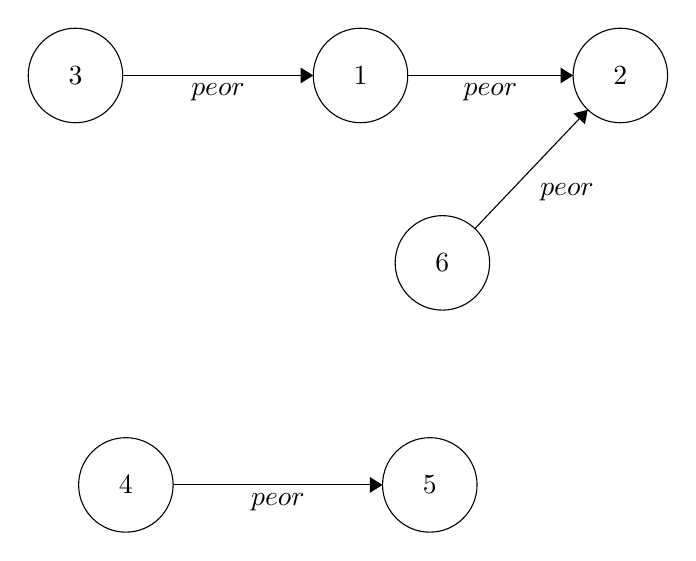
\begin{tikzpicture}[scale=0.2]
        \tikzstyle{every node}+=[inner sep=0pt]
        \draw [black] (36.4,-11.9) circle (3);
        \draw (36.4,-11.9) node {$1$};
        \draw [black] (52.9,-11.9) circle (3);
        \draw (52.9,-11.9) node {$2$};
        \draw [black] (18.3,-11.9) circle (3);
        \draw (18.3,-11.9) node {$3$};
        \draw [black] (41.6,-23.8) circle (3);
        \draw (41.6,-23.8) node {$6$};
        \draw [black] (21.5,-37.9) circle (3);
        \draw (21.5,-37.9) node {$4$};
        \draw [black] (40.8,-37.9) circle (3);
        \draw (40.8,-37.9) node {$5$};
        \draw [black] (39.4,-11.9) -- (49.9,-11.9);
        \fill [black] (49.9,-11.9) -- (49.1,-11.4) -- (49.1,-12.4);
        \draw (44.65,-12.4) node [below] {$peor$};
        \draw [black] (21.3,-11.9) -- (33.4,-11.9);
        \fill [black] (33.4,-11.9) -- (32.6,-11.4) -- (32.6,-12.4);
        \draw (27.35,-12.4) node [below] {$peor$};
        \draw [black] (43.67,-21.62) -- (50.83,-14.08);
        \fill [black] (50.83,-14.08) -- (49.92,-14.31) -- (50.65,-15);
        \draw (47.78,-19.32) node [right] {$peor$};
        \draw [black] (24.5,-37.9) -- (37.8,-37.9);
        \fill [black] (37.8,-37.9) -- (37,-37.4) -- (37,-38.4);
        \draw (31.15,-38.4) node [below] {$peor$};
        \end{tikzpicture}
    \end{center}
\end{figure}

Si quiero saber si X es peor que Y pero no lo tengo directo ¿Que puedo hacer? podemos pararnos en la arista X y ver si puedo llegar a la arista Y. \break 
Se de una arista no puedo llegar a otra quiere decir que no es una verdad, pero debemos ver si es un alternative Fact, esto lo logramos inviertiendo nuestra búsqueda si buscamos desde Y a X y se cumple tenemos un alternative fact.\break 
Finalmente si ninguno de los dos se cumple imprimimos Pants on fire. \break 
¿Que pasa si no conocemos una nacionalidad? Si no esta en nuestro diccionaro es una mentira por tanto mandamos Pants on fire, es decir ni existe. \break 

Para implementar que ¿podemos hacer?

\begin{lstlisting}
    #include <bits/stdc++.h>

    using namespace std;

    map<string, int> dictionary;
    vector< vector<int> > adjList;
    vector< bool > visited;
    
    bool DFS( int u, int v ){
        bool ans = false;
        if( u == v )
            return true;
        visited[ u ] = true;
        for( int i = 0; i < adjList[ u ].size(); i++ ){
            int w = adjList[ u ][ i ];
            if( !visited[ w ] ){
                if( DFS( w, v ) ){
                    ans = true;
                    break;
                }
            }
        }
        return ans;
    }

    int main(){
        int count = 0;
        int m, n, u, v, a, b;
        cin >> m >> n;
        for( int i = 0; i < m; i++ ){
            cin >> a >> b;
            if( dictionary.find( a ) != dictionary.end() )
                u = dictionary[ a ];
            else 
                u = dictionary[ a ] = count++;
            if( dictionary.find( b ) != dictionary.end() )
                v = dictionary[ b ];
            else 
                v = dictionary[ b ] = count++;
            //Enlazamos los nodos (creamos el grafo)
            adj[ u ].push_back( v );
        }
        //Procesamos las queries
        for( int i = 0; i < n; i++ ){

            //Extraemos los IDs 
            cin >> a >> b;
            //Buscamos el ID de la primer nacionalidad
            if( dictionary.find( a ) != dictionary.end() )
                u = dictionary[ a ];
            //Buscamos el ID de la segunda nacionalidad
            if( dictionary.find( b ) != dictionary.end() )
                v = dictionary[ b ];

            //Se cumplió totalmente lo que se ha dicho
            if( DFS(u, v) )
                cout << "Fact\n";
            //Si invertimos se cumple
            else if( DFS(v, u) )
                cout << "Alternative fact\n";
            //No es verdad
            else 
                cout << "Paths on fire\n";
        }
        return 0;
    }
\end{lstlisting}

\chapter{Teoría de números}
Recordemos los conjuntos de números 
\begin{itemize}
    \item Números enteros: $Z = {..., -3, -2, -1, 0, 1, 2, 3, ... }$
    \item Números naturales/Números positivos $N = {1, 2, 3, ..., }$
\end{itemize}

\section{Divisibilidad}
\textbf{d} divide a \textbf{a} si existe un entero \textbf{q} tal que $a = dq$, y se escribe $d|a$\newline
\textit{Ejemplos:}\break 
\begin{itemize}
    \item {$2|6 \rightarrow 6 = 2(3)$}
    \item {$5|6 \rightarrow 6 = 5(q), q = 1.2$}
\end{itemize}

\subsection{Algoritmo de la división}
Sean \textbf{$a,b \epsilon Z$}. Entonces existen \textbf{$q, e \epsilon Z$} tal que:\newline
\[ a = bq + r \]
donde: $0 \leq r < |b|$ \newline

\textit{Ejemplo} \newline
a = 15, b = 6 \newline 
15 = 6(2) + 3 \newline 
dónde: 
\begin{itemize}
    \item {El cociente = 2}
    \item {El residuo = 3}
\end{itemize}

De forma general 
\[
    q = piso \left ( \frac{a}{b} \right )
\]

Y también 
\[
    r = a \% b    
\]

\subsubsection{¿Cómo hallar los divisores de un número?}
\begin{lstlisting}
    vector< int > divisores( int n ){
        vector< int > div;
        for( int d = 1; d <= n; d++)
            if( n % d == 0 )
                div.push_back( d );
        return div;
    }
\end{lstlisting}
La complejidad del algoritmo anterior es $O(n)$ siendo así vamos a tratar de optimizar esta función\newline

Que pasa si queremos los divisores de un n = 24, los divisores de este número son $\{1, 2, 3, 4, 6, 8, 12, 24\}$ podemos observar que siempre los divisores van en ''parejas'' es decir siempre tenemos lo siguiente: \newline
\begin{itemize}
    \item {d = 1, q = 24}
    \item {d = 2, q = 12}
    \item {d = 3, q = 8}
    \item {d = 4, q = 6}
\end{itemize}

Además sabemos que n = dq por tanto \newline
\[ d \leq q \]
\[ d^{2} \leq dq \]
\[ \sqrt{d^{2}} \leq \sqrt{n} \]
\[ d \leq \sqrt{n} \]

¿En código que obtenemos?

\begin{lstlisting}
    vector< int > divisores( int n ){
        vector< int > div;
        for( int d = 1; d *d <= n; d++){
            if( n % d == 0 ){
                int q = n / d;
                div.push_back( d );
                //Para evitar números repqtidos, analizar el caso del 25
                if( q != d)
                    div.push_back( q );
            }
        }
        return div;
    }
\end{lstlisting}

La complejidad de este algoritmo es de $O(\sqrt{n})$ \newline

Que pasa si hacemos uso de números negativos ¿Qué sucede?

\[ int a = -13, b = 4\]
\[ int q = \frac{a}{b} \]
\[ int r = a \% b \]
\[ a = bq + r\]
\[ -13 = 4(-3) + (-1)\]
\[ -13 = -12 - 1\]
Lo cual no es del todo correcto ya que nuestro residuo debería ser 3
\[ -13 = 4(-4) + 3\]
\[ -13 = -16 + 3\]
¿Como reparamos esto?
\begin{lstlisting}
    if( r < 0 )
        r += b
\end{lstlisting}

\section{Números primos}

Sea $p \epsilon N$ con $p \geq 2$ p es primo si: sus unicos divisores son 1 y p.

\subsection{Test de primalidad}
¿Cómo puedo saber si un n es primo?
\begin{lstlisting}
    bool esPrimo( int n ){
        if( n < 2 )
            return false;

        for( int d = 2; d*d <= n; d++ )
            if( n % q == 0 )
                return false;
        return true;
    }
\end{lstlisting}
La complejidad de este algoritmo es $O(\sqrt{n})$

\subsubsection{Problema}
\textbf{Hallar todos los primos menores o iguales a n \newline Ejemplo: }
$ n = 10 \rightarrow \{ 2, 3, 5, 7 \}$ \newline

\begin{lstlisting}
    vector< int > primos;
    for( int d = 2; d <= n; d++ ){
        if( esPrimo( d ) )
            primos.push_back( d );
    }
\end{lstlisting}

La complejidad de este algoritmo es $O(n \sqrt{n})$ en este caso a lo mucho podríamos procesar en un segundo si $n \leq 5 * 10^{5}$

\section{Criba de eratóstenes}
En este caso nos ''paramos'' en un número y ''marcamos'' todos sus múltiplos. \newline

Empezamos con el 2
\begin{figure}[H]
\begin{longtable}[c]{|
    >{\columncolor[HTML]{EFEFEF}}l |
    >{\columncolor[HTML]{FFFFFF}}l |
    >{\columncolor[HTML]{FFFFFF}}l |
    >{\columncolor[HTML]{FFFFFF}}l |
    >{\columncolor[HTML]{FFFFFF}}l |
    >{\columncolor[HTML]{FFFFFF}}l |
    >{\columncolor[HTML]{FFFFFF}}l |
    >{\columncolor[HTML]{FFFFFF}}l |
    >{\columncolor[HTML]{FFFFFF}}l |
    >{\columncolor[HTML]{FFFFFF}}l |
    >{\columncolor[HTML]{FFFFFF}}l |
    >{\columncolor[HTML]{FFFFFF}}l |
    >{\columncolor[HTML]{FFFFFF}}l |
    >{\columncolor[HTML]{FFFFFF}}l |
    >{\columncolor[HTML]{FFFFFF}}l |
    >{\columncolor[HTML]{FFFFFF}}l |
    >{\columncolor[HTML]{FFFFFF}}l |
    >{\columncolor[HTML]{FFFFFF}}l |
    >{\columncolor[HTML]{FFFFFF}}l |}
    \hline
    {\color[HTML]{333333} 2} & {\color[HTML]{333333} 3} & {\color[HTML]{333333} 4} & {\color[HTML]{333333} 5} & {\color[HTML]{333333} 6} & {\color[HTML]{333333} 7} & {\color[HTML]{333333} 8} & {\color[HTML]{333333} 9} & {\color[HTML]{333333} 10} & {\color[HTML]{333333} 11} & {\color[HTML]{333333} 12} & {\color[HTML]{333333} 13} & 14 & 15 & 16 & 17 & 18 & 19 & 20 \\ \hline
    \endfirsthead
    %
    \endhead
    %
    \cellcolor[HTML]{FFFFFF} & {\color[HTML]{C0C0C0} } & x &  & x &  & x &  & x &  & x &  & x &  & x &  & x &  & x \\ \hline
    \end{longtable}
\end{figure}

Nos paramos en el 3
\begin{figure}[H]
\begin{longtable}[c]{|
    >{\columncolor[HTML]{EFEFEF}}l |
    >{\columncolor[HTML]{EFEFEF}}l |
    >{\columncolor[HTML]{FFFFFF}}l |
    >{\columncolor[HTML]{FFFFFF}}l |
    >{\columncolor[HTML]{FFFFFF}}l |
    >{\columncolor[HTML]{FFFFFF}}l |
    >{\columncolor[HTML]{FFFFFF}}l |
    >{\columncolor[HTML]{FFFFFF}}l |
    >{\columncolor[HTML]{FFFFFF}}l |
    >{\columncolor[HTML]{FFFFFF}}l |
    >{\columncolor[HTML]{FFFFFF}}l |
    >{\columncolor[HTML]{FFFFFF}}l |
    >{\columncolor[HTML]{FFFFFF}}l |
    >{\columncolor[HTML]{FFFFFF}}l |
    >{\columncolor[HTML]{FFFFFF}}l |
    >{\columncolor[HTML]{FFFFFF}}l |
    >{\columncolor[HTML]{FFFFFF}}l |
    >{\columncolor[HTML]{FFFFFF}}l |
    >{\columncolor[HTML]{FFFFFF}}l |}
    \hline
    {\color[HTML]{333333} 2} & {\color[HTML]{333333} 3} & {\color[HTML]{333333} 4} & {\color[HTML]{333333} 5} & {\color[HTML]{333333} 6} & {\color[HTML]{333333} 7} & {\color[HTML]{333333} 8} & {\color[HTML]{333333} 9} & {\color[HTML]{333333} 10} & {\color[HTML]{333333} 11} & {\color[HTML]{333333} 12} & {\color[HTML]{333333} 13} & 14 & 15 & 16 & 17 & 18 & 19 & 20 \\ \hline
    \endfirsthead
    %
    \endhead
    %
    \cellcolor[HTML]{FFFFFF} & \cellcolor[HTML]{FFFFFF}{\color[HTML]{C0C0C0} } & x &  & x &  & x & x & x &  & x &  & x & x & x &  & x &  & x \\ \hline
    \end{longtable}
\end{figure}

Nos paramos en el 4
\begin{figure}[H]
\begin{longtable}[c]{|
    >{\columncolor[HTML]{EFEFEF}}l |
    >{\columncolor[HTML]{EFEFEF}}l |
    >{\columncolor[HTML]{EFEFEF}}l |
    >{\columncolor[HTML]{FFFFFF}}l |
    >{\columncolor[HTML]{FFFFFF}}l |
    >{\columncolor[HTML]{FFFFFF}}l |
    >{\columncolor[HTML]{FFFFFF}}l |
    >{\columncolor[HTML]{FFFFFF}}l |
    >{\columncolor[HTML]{FFFFFF}}l |
    >{\columncolor[HTML]{FFFFFF}}l |
    >{\columncolor[HTML]{FFFFFF}}l |
    >{\columncolor[HTML]{FFFFFF}}l |
    >{\columncolor[HTML]{FFFFFF}}l |
    >{\columncolor[HTML]{FFFFFF}}l |
    >{\columncolor[HTML]{FFFFFF}}l |
    >{\columncolor[HTML]{FFFFFF}}l |
    >{\columncolor[HTML]{FFFFFF}}l |
    >{\columncolor[HTML]{FFFFFF}}l |
    >{\columncolor[HTML]{FFFFFF}}l |}
    \hline
    {\color[HTML]{333333} 2} & {\color[HTML]{333333} 3} & {\color[HTML]{333333} 4} & {\color[HTML]{333333} 5} & {\color[HTML]{333333} 6} & {\color[HTML]{333333} 7} & {\color[HTML]{333333} 8} & {\color[HTML]{333333} 9} & {\color[HTML]{333333} 10} & {\color[HTML]{333333} 11} & {\color[HTML]{333333} 12} & {\color[HTML]{333333} 13} & 14 & 15 & 16 & 17 & 18 & 19 & 20 \\ \hline
    \endfirsthead
    %
    \endhead
    %
    \cellcolor[HTML]{FFFFFF} & \cellcolor[HTML]{FFFFFF}{\color[HTML]{C0C0C0} } & \cellcolor[HTML]{FFFFFF}x &  & x &  & x & x & x &  & x &  & x & x & x &  & x &  & x \\ \hline
    \end{longtable}
\end{figure}

Ya hemos hecho lo mismo con los 20 números
\begin{figure}[H]
\begin{longtable}[c]{|l|l|l|l|l|l|l|l|l|l|l|l|l|l|l|l|l|l|l|}
    \hline
    \rowcolor[HTML]{EFEFEF} 
    {\color[HTML]{333333} 2} & {\color[HTML]{333333} 3} & {\color[HTML]{333333} 4} & {\color[HTML]{333333} 5} & {\color[HTML]{333333} 6} & {\color[HTML]{333333} 7} & {\color[HTML]{333333} 8} & {\color[HTML]{333333} 9} & {\color[HTML]{333333} 10} & {\color[HTML]{333333} 11} & {\color[HTML]{333333} 12} & {\color[HTML]{333333} 13} & 14 & 15 & 16 & 17 & 18 & 19 & 20 \\ \hline
    \endfirsthead
    %
    \endhead
    %
    \rowcolor[HTML]{FFFFFF} 
     & {\color[HTML]{C0C0C0} } & x &  & x &  & x & x & x &  & x &  & x & x & x &  & x &  & x \\ \hline
    \end{longtable}
\end{figure}

¿En código como sería esto?

\begin{lstlisting}
    vector< int > criba( int n ){
        vector< bool > esPrimo( n + 1, true );
        vector< int > factoresPrimos;
        factoresPrimos.push_back( 2 );
        for( int i = 4; i <= n; i += 2 )
            esPrimo[ i ] = false;
        
        for( int i = 3; i <= n; i++ ){
            if( esPrimo[ i ] ){
                factoresPrimos.push_back( i );
                for( int j = i * 2; j <= n; j += i ){
                    esPrimo[ j ] = false;
                }
            }
        }
    }
\end{lstlisting}

La complejidad de este algoritmo ¿cual es? $O\left ( n + \frac{n}{2} + \frac{n}{3} + ... + \frac{n}{n} \right )$ lo que es igual a $O\left ( \sum_{i = 1}^{n}( \frac{ n }{ i }) \right )$ si opeamos $O\left ( n \sum_{ i = 2 }^{ n } \frac{ 1 }{ i } \right )$ asintóticamente esta suma es igual a $log(n)$ es decir la complejidad de este algoritmo es $O(nlog(n))$ la complejidad espacial (en memoria) es $O(n)$ lo cual es muy bueno si $n \leq 10^{ 7 } $ Podemos optimizar un poco máscaras
\begin{lstlisting}
    vector< int > criba( int n ){
        vector< bool > esPrimo( n + 1, true );
        vector< int > factoresPrimos;
        factoresPrimos.push_back( 2 );
        for( int i = 4; i <= n; i += 2 )
            esPrimo[ i ] = false;
        
        for( int i = 3; i <= n; i++ ){
            if( esPrimo[ i ] ){
                factoresPrimos.push_back( i );
                //Iniciamos en i * i no en i * 2
                for( int j = i * i; j <= n; j += i ){
                    esPrimo[ j ] = false;
                }
            }
        }
    }
\end{lstlisting}

La complejidad de esta $O( nlog(log(n)))$ podemos mejorarla un poco más 

\begin{lstlisting}
    vector< int > criba( int n ){
        vector< bool > esPrimo( n + 1, true );
        vector< int > factoresPrimos;
        factoresPrimos.push_back( 2 );
        for( int i = 4; i <= n; i += 2 )
            esPrimo[ i ] = false;
        
        for( int i = 3; i <= n; i++ ){
            if( esPrimo[ i ] ){
                factoresPrimos.push_back( i );
                //Incrementamos en j += 2*i
                for( int j = i * i; j <= n; j += 2 * i ){
                    esPrimo[ j ] = false;
                }
            }
        }
    }
\end{lstlisting}

\section{Obtención de factores primos}
Ya conocemos la criba, con la misma podemos obtener otra información. En esta ocasión vamos a obtener el factor primo más pequeño de un número. En este caso utilizaremos un arreglo de booleanos. \newline

Un factor primo recordemos que se puede definir de la siguiente forma
\[
    N = P_{1}^{\alpha_{1}} P_{2}^{\alpha_{2}} ... P_{k}^{\alpha_{k}}
\]
Por ejemplo, ¿Cuál es la factorización prima del 36? \newline

\[ 36 = 2^{2}3^{2} \]

Esto también es comocido como el teorema fundamental de la aritmética. También es importante saber que esta factorización es \textbf{única}. \newline
También consideremos que el factor primo de un número primo es si mismo. Por ejemplo los factores primos del 3 es el 3 mismo. \newline
Tenemos varios algoritmos para obtener el factor primo más pequeño, nosotros usaremos el siguiente:
\begin{lstlisting}
    vector< int > lowestPrime( n + 1 );
    //Marcamos todos los pares 
    for( int i = 2; i <= n; i += 2 )
        lowestPrime[ i ] = 2;
    //Recorremos todos los impares 
    for( int i = 3; i <= n; i += 2 ){
        //No se ha marcado aún
        if( lowestPrime[ i ] == 0 ){
            lowestPrime[ i ] = i;
            for( int j = i * i; j <= n; j+= 2 ){
                //Quizá alguien ya lo marcó, por tanto preguntamos si esta disponible para usar
                if( lowestPrime[ j ] == 0 )
                    lowestPrime[ j ] = i;
            }
        }
    }
\end{lstlisting}

Este algoritmo tiene una complejidad de $O(nln(n))$

Ahora vamos a obtener la descomposición prima de un número n, si lo hacemos en papel, podemos construir una tabla, nuevamente tomemos de ejemplo al 36
\begin{figure}[H]
    \begin{longtable}[c]{|l|l|}
    \hline
    \rowcolor[HTML]{C0C0C0} 
    {\color[HTML]{333333} 36} & {\color[HTML]{333333} 2} \\ \hline
    \endfirsthead
    %
    \endhead
    %
    \rowcolor[HTML]{FFFFFF} 
    18 & {\color[HTML]{333333} 2} \\ \hline
    \rowcolor[HTML]{FFFFFF} 
    9 & 3 \\ \hline
    \rowcolor[HTML]{FFFFFF} 
    3 & 3 \\ \hline
    \rowcolor[HTML]{FFFFFF} 
    1 &  \\ \hline
    \end{longtable}
\end{figure}

\begin{lstlisting}
    vector< int > factorizar( int n ){
        vector< int > factor;
        while( n > 1 ){
            int p = lowestPrime[ n ];
            factor.push_back( p );
            n /= p;
        }
        return factor;
    }
\end{lstlisting}

La complejidad de obtener los factores primos es aproximadamente $O( n_{}primos )$ esto es aproximadamente $O(log_{2}(n))$ \newline

¿Cómo podemos obtener los primos cuya potencia es par?

\begin{lstlisting}
    #define vector<int, int> pii;
    vector< pii > factorizar( int n ){
        vector< pii > factor;
        while( n > 1 ){
            int p = lowestPrime[ n ];
            int pow = 0;
            while( n % p == 0 )
                n /= p, pow++;
            //emplace_back llama al constructor de pair
            factor.emplace_back( p, pow );
            
        }
        return factor;
    }
\end{lstlisting}

Otra característica de los números enteros es que los divisores de un n tienen los mismos divisores primos pero con potencias diferentes. Por ejemplo, nuevamente para el 36:
\begin{figure}[H]
    \begin{longtable}[c]{|
    >{\columncolor[HTML]{FFFFFF}}l |
    >{\columncolor[HTML]{FFFFFF}}l |}
    \hline
    {\color[HTML]{333333} 1} & {\color[HTML]{333333} } \\ \hline
    \endfirsthead
    %
    \endhead
    %
    2 & {\color[HTML]{333333} } \\ \hline
    3 &  \\ \hline
    4 & $2^{2}3^{0}$\\ \hline
    6 &  \\ \hline
    9 &  \\ \hline
    12 & $2^{2}3^{3}$ \\ \hline
    18 &  \\ \hline
    36 &  \\ \hline
    \end{longtable}
\end{figure}

Más formalmente 

\[
    N = P_{1}^{\alpha_{1}} P_{2}^{\alpha_{2}} ... P_{k}^{\alpha_{k}}   
\]

x divide a N 

\[
    x = P_{1}^{\beta_{1}} P_{2}^{\beta_{2}} ... P_{k}^{\beta_{k}}
\]

\[
  \beta_{1} \leq \alpha_{1}, \beta_{2} \leq \alpha_{2},..., \beta_{k} \leq \alpha_{k}
\]

\section{Ejercicio}
\textbf{Dados factores primos y sus potencias, hallar todos los divisores de N $N \leq 10^{18}$ } \newline 
\textbf{Ejemplo:}\newline
N = 36 \newline
2, 2 \newline 
3, 2 \newline
El Output sería \newline
Res = 1, 2, 3, 4, 6,... , 36 \newline
\textsf{Solución:}\newline
Sabemos del teorema fundamental del cálculo que las potencias a las que estan elevados los números primos (factores de nuestro número N). Haciendo uso de ese hecho podemos iterar sobre todas las potencias que nos dan, desde cero hasta la k potencia. En código podemos probar todas las combinaciones de forma recursiva.

\begin{lstlisting}
    #define pair< int, int > pii
    .
    .
    .
    vector< int > divisors;
    //Aquí vamos a guardar los números y sus potencias
    vector< pii > factors;

    void findDivisors( int index, int current_product ){

        //Guardamos el divisor
        if( index == factors.size() )
            divisors.push_back( current_product );

        for( int i = 0; i <= factors[ index ].second; i++ ){
            findDivisors( index + 1, current_product * pow( factors[ index ].first, i ) );
        }
            
    }
    .
    .
    .
    int main(){
        pii factor;
        for( int i = 0; i < k; i++ ){
            //first = número primo 
            //second = la potencia
            cin >> factor.first >> factor.second;
            factors.push_back( factor );
        }
    }
\end{lstlisting}

Si dibujamos las llamadas recursivas tendríamos algo como esto
\begin{figure}[H]
    \begin{center}
        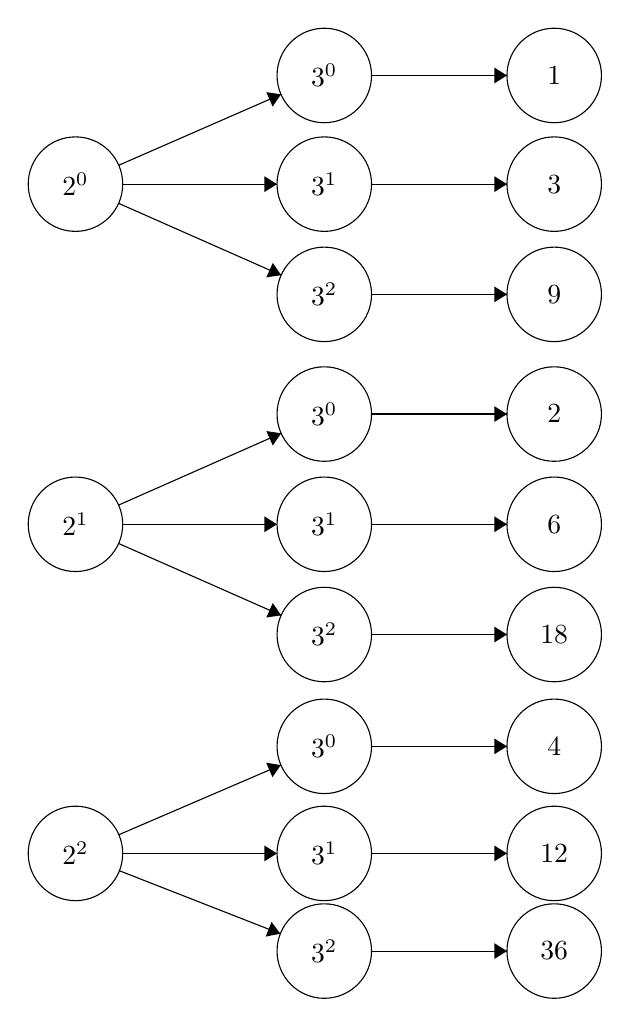
\begin{tikzpicture}[scale=0.2]
        \tikzstyle{every node}+=[inner sep=0pt]
        \draw [black] (14.5,-10) circle (3);
        \draw (14.5,-10) node {$2^{0}$};
        \draw [black] (14.5,-31.6) circle (3);
        \draw (14.5,-31.6) node {$2^{1}$};
        \draw [black] (30.3,-45.7) circle (3);
        \draw (30.3,-45.7) node {$3^{0}$};
        \draw [black] (30.3,-3.1) circle (3);
        \draw (30.3,-3.1) node {$3^{0}$};
        \draw [black] (30.3,-10) circle (3);
        \draw (30.3,-10) node {$3^{1}$};
        \draw [black] (30.3,-17) circle (3);
        \draw (30.3,-17) node {$3^{2}$};
        \draw [black] (30.3,-24.6) circle (3);
        \draw (30.3,-24.6) node {$3^{0}$};
        \draw [black] (30.3,-31.6) circle (3);
        \draw (30.3,-31.6) node {$3^{1}$};
        \draw [black] (30.3,-38.6) circle (3);
        \draw (30.3,-38.6) node {$3^{2}$};
        \draw [black] (30.3,-52.5) circle (3);
        \draw (30.3,-52.5) node {$3^{1}$};
        \draw [black] (30.3,-58.7) circle (3);
        \draw (30.3,-58.7) node {$3^{2}$};
        \draw [black] (14.5,-52.5) circle (3);
        \draw (14.5,-52.5) node {$2^{2}$};
        \draw [black] (44.9,-3.1) circle (3);
        \draw (44.9,-3.1) node {$1$};
        \draw [black] (44.9,-10) circle (3);
        \draw (44.9,-10) node {$3$};
        \draw [black] (44.9,-17) circle (3);
        \draw (44.9,-17) node {$9$};
        \draw [black] (44.9,-24.6) circle (3);
        \draw (44.9,-24.6) node {$2$};
        \draw [black] (44.9,-31.6) circle (3);
        \draw (44.9,-31.6) node {$6$};
        \draw [black] (44.9,-38.6) circle (3);
        \draw (44.9,-38.6) node {$18$};
        \draw [black] (44.9,-45.7) circle (3);
        \draw (44.9,-45.7) node {$4$};
        \draw [black] (44.9,-52.5) circle (3);
        \draw (44.9,-52.5) node {$12$};
        \draw [black] (44.9,-58.7) circle (3);
        \draw (44.9,-58.7) node {$36$};
        \draw [black] (17.25,-8.8) -- (27.55,-4.3);
        \fill [black] (27.55,-4.3) -- (26.62,-4.16) -- (27.02,-5.08);
        \draw [black] (17.5,-10) -- (27.3,-10);
        \fill [black] (27.3,-10) -- (26.5,-9.5) -- (26.5,-10.5);
        \draw [black] (17.24,-11.22) -- (27.56,-15.78);
        \fill [black] (27.56,-15.78) -- (27.03,-15) -- (26.62,-15.92);
        \draw [black] (17.24,-30.38) -- (27.56,-25.82);
        \fill [black] (27.56,-25.82) -- (26.62,-25.68) -- (27.03,-26.6);
        \draw [black] (17.5,-31.6) -- (27.3,-31.6);
        \fill [black] (27.3,-31.6) -- (26.5,-31.1) -- (26.5,-32.1);
        \draw [black] (17.24,-32.82) -- (27.56,-37.38);
        \fill [black] (27.56,-37.38) -- (27.03,-36.6) -- (26.62,-37.52);
        \draw [black] (17.26,-51.31) -- (27.54,-46.89);
        \fill [black] (27.54,-46.89) -- (26.61,-46.74) -- (27.01,-47.66);
        \draw [black] (17.5,-52.5) -- (27.3,-52.5);
        \fill [black] (27.3,-52.5) -- (26.5,-52) -- (26.5,-53);
        \draw [black] (17.29,-53.6) -- (27.51,-57.6);
        \fill [black] (27.51,-57.6) -- (26.95,-56.85) -- (26.58,-57.78);
        \draw [black] (33.3,-3.1) -- (41.9,-3.1);
        \fill [black] (41.9,-3.1) -- (41.1,-2.6) -- (41.1,-3.6);
        \draw [black] (33.3,-10) -- (41.9,-10);
        \fill [black] (41.9,-10) -- (41.1,-9.5) -- (41.1,-10.5);
        \draw [black] (33.3,-17) -- (41.9,-17);
        \fill [black] (41.9,-17) -- (41.1,-16.5) -- (41.1,-17.5);
        \draw [black] (33.3,-24.6) -- (41.9,-24.6);
        \fill [black] (41.9,-24.6) -- (41.1,-24.1) -- (41.1,-25.1);
        \draw [black] (33.3,-31.6) -- (41.9,-31.6);
        \fill [black] (41.9,-31.6) -- (41.1,-31.1) -- (41.1,-32.1);
        \draw [black] (33.3,-38.6) -- (41.9,-38.6);
        \fill [black] (41.9,-38.6) -- (41.1,-38.1) -- (41.1,-39.1);
        \draw [black] (33.3,-45.7) -- (41.9,-45.7);
        \fill [black] (41.9,-45.7) -- (41.1,-45.2) -- (41.1,-46.2);
        \draw [black] (33.3,-52.5) -- (41.9,-52.5);
        \fill [black] (41.9,-52.5) -- (41.1,-52) -- (41.1,-53);
        \draw [black] (33.3,-58.7) -- (41.9,-58.7);
        \fill [black] (41.9,-58.7) -- (41.1,-58.2) -- (41.1,-59.2);
        \end{tikzpicture}
    \end{center}
\end{figure}

\section{Máximo Común Divisor (GCD)}
La notación ha utilizar será GCD(a, b) = g, dónde:
\begin{itemize}
    \item {$g$ divide a $a$}
    \item {$g$ divide a $b$}
    \item {$g$ es el máximo entero que cumple las propiedades}
\end{itemize}

Por ejemplo, ¿Cuáles son los divisores comúnes de 48 y 72? \newline
$\{ 1, 2, 3, 4, 6, 8, 12, 24 \}$ \newline
El divisor común con valor mayor es el 24, este es el GCD(48, 72) \newline
\paragraph{Algunas propiedades}
\begin{itemize}
    \item {El GCD entre 0 y N es N es decir $GCD(0, N) = N$}
    \item {El GCD entre 1 y N es 1 es decir $GCD(1, N) = 1$}
    \item {El GCD entre N y N + 1 siempre es 1 es decir $GCD(N, N + 1) = 1$}
    \item {Si el GCD entre a y b es igual con 1 esos números son comprimos es decir $GCD(A, B) = 1$}
    \item {EL GCD entre un primo $P_{1}$ y un primo $P_{2}$ siempre es 1 ya que ambos números tienen como único divisor y el número mismo, por tanto el único divisor común es 1 es decir $GCD(P_{1}, P_{2}) = 1$}
\end{itemize}

\subsection{Algoritmo de Euclides}
Dado un número a y un número b, ¿Cómo podemos encontrar su GCD?
\begin{lstlisting}
    int Euclides( int a, int b ){
        if( a > b )
            swap(a, b);
        while( a != 0 ){
            b %= a;
            swap(a, b)
        }
        return b;
    }
\end{lstlisting}
Lo anterior sirve si y solo si 
Si $a > b$ \newline
Si se cumple esa condición sabemos que siempre:
$b \% a < a$ \newline
También existe una desigualdad la cual dice que:
$b \% a \leq \frac{b}{2}$ \newline
La cual es demostrable si separamos en dos casos:
\begin{enumerate}
    \item {$a \leq \frac{b}{2}$}
    \item {$a > \frac{b}{2}$}
\end{enumerate}

Otra versión del algoritmo de euclides es:

\begin{lstlisting}
    int Euclides( int a, int b ){
        return a ? ( b % a, a ) : b;
    }
\end{lstlisting}

Si usamos C++ podemos usar 

\begin{lstlisting}
    g = __gcd(a, b);
\end{lstlisting}

\section{Mínimo común multiplo (LCM)}
Dados dos números a y b se cumple que:
\begin{itemize}
    \item {$a$ divide a $l$}
    \item {$b$ divide a $l$}
    \item {$l$ es el menor entero que cumple}
\end{itemize}
\textsf{Ejemplo}\newline
El MCM entre 10 y 15 es el 30 ya que:
\begin{itemize}
    \item {$\frac{10}{30} = 3$}
    \item {$\frac{15}{30} = 2$}
\end{itemize}
¿Como obtenemos esto? consideremos que 
\[
    a * b = GCD(a, b) * LCM(a, b);
\]
Despejando 
\[
    LCM(a, b) = \frac{a * b}{GCD(a, b)}
\]
También debemos preguntarnos ¿Cómo es que $a * b = GCD(a, b) * LCM(a, b);$ es verdad? \newline
Sea:
\begin{itemize}
    \item {$a = P_{1}^{\alpha_{1}}P_{2}^{\alpha_{2}}...P_{k}^{\alpha_{k}}$}
    \item {$b = P_{1}^{\beta{1}}P_{2}^{\beta{2}}...P_{k}^{\beta{k}}$}
    \item {$g = P_{1}^{\gamma{1}}P_{2}^{\gamma{2}}...P_{k}^{\gamma{k}}$}
\end{itemize}
Sabemos que las potencias $\alpha$ seran menores que las potencias de $\gamma$ lo mismo con las potencias de $\beta$, es decir:
\begin{itemize}
    \item {$\gamma_{k} \leq \alpha_{k}$}
    \item {$\gamma_{k} \leq \beta_{k}$}
\end{itemize}
El GCD lo obtenemos de el mínimo entre ambas potencias es decir \newline
$\gamma_{k} = min(\alpha_{k}, \beta_{k})$ \newline
Mientras que el LCM lo obtenemos de entre el máximo de las potencias, tomemos en cuenta que 
\begin{itemize}
    \item {$a = P_{1}^{\alpha_{1}}P_{2}^{\alpha_{2}}...P_{k}^{\alpha_{k}}$}
    \item {$b = P_{1}^{\beta{1}}P_{2}^{\beta{2}}...P_{k}^{\beta{k}}$}
    \item {$l = P_{1}^{\pi_{1}}P_{2}^{\pi_{2}}...P_{k}^{\pi_{k}}$}
\end{itemize}
Nuevamente
\begin{itemize}
    \item {$\pi_{k} \leq \alpha_{k}$}
    \item {$\pi_{k} \leq \beta_{k}$}
\end{itemize}
El LCM lo obtenemos de el máximo entre ambas potencias es decir: \newline
$\pi_{k} = min(\alpha_{k}, \beta_{k})$ \newline

Si utilizamos la definición de LCM que mencionamos anteriormente pero sustituyendo los valores: \newline
$a * b = (P_{1}^{\alpha_{1}}P_{2}^{\alpha_{2}}...P_{k}^{\alpha_{k}})(P_{1}^{\beta{1}}P_{2}^{\beta{2}}...P_{k}^{\beta{k}})$ \newline
Esto es igual a la suma de las potencias es decir 
$P_{1}^{\alpha_{1} + \beta_{1}}P_{2}^{\alpha_{2} + \beta_{2}}...P_{k}^{\alpha_{k} + \beta_{k}}$\newline
Por tanto \newline
$GCD(a, b)*LCM(a, b) = \left ( P_{1}^{ min(\alpha_{1}, \beta_{1})} \dots P_{k}^{ min(\alpha_{k}, \beta_{k}) }  \right )$

\section{Aritmética modular}
Anteriormente se ha utilizado el módulo para saber por ejemplo si un número es par o impar, es decir hacemos:
\begin{lstlisting}
    if( (a % 2) == 0 )
        cout << "Es par" << endl;
    else 
        cout << "Es impar" << endl;
\end{lstlisting}
Formalmente el módulo lo definimos como \newline
\[
    a = b * q + r
\]

dónde:
\begin{itemize}
    \item a = número 
    \item b = módulo 
    \item q = entero multiplicado tal que nos da un valor igual o menos que el a
    \item r = residuo
\end{itemize}

Por ejemplo si tenemos el 7 

\[
    7 = 2 * 3 + 1
\]

Entonces el módulo es el residuo de una división. Esto solo aplica a números enteros no para reales. El módulo nos forma familias, las familias son cíclicas. También debemos mencionar que al aplicar módulo n obtendremos un número que está entre $[ 0, 1, 2, \dots, n - 1 ]$ 

\subsection{Congruencia}
Un número es congruente si se cumple que:
\[
    n \equiv a mod b
\]
Por ejemplo los números pares
\[
    4 mod 2 = 0
\]
\[
    6 mod 2 = 0
\]

Estos siempre ''viven'' en las mismas familias \newline

\subsection{Operaciones}
\subsubsection{Suma}
Supongamos que tenemos lo siguiente
\[
    (a + b) \% N    
\]

Podemos representar esto como 
\[
    ( ( a \% n ) + ( b \% n ) ) \% n    
\]

Siempre debemos de modular después de una suma ya que si no modulamos nos saldríamos de la familia en la que estamos.

\subsubsection{Multiplicación}
\[
    (a + b) \% N    
\]

Podemos representar esto como 
\[
    ( ( a \% n ) * ( b \% n ) ) \% n    
\]

\subsection{Inverso modular}
Ya sabemos que exite la suma y la multiplicación modular, pero ¿existe la división? realmente no hay una definición para esto, pero si sabemos que:
\[
    \frac{a}{b} = a*b^{-1}    
\]
Sabiendo esto y también conociendo la regla de congruencia, podemos calcular ese $b^{-1}$ es decir:
\[
    a * x \equiv 1 mod N    
\]
\[
    a * a^{-1} \equiv 1 mod N    
\]

\section{Exponenciación binaria}
Hasta ahora sabemos que podemos exponenciar un número $n$ a una potencia $b$ es decir 
\begin{lstlisting}
    pow(n, b);
\end{lstlisting}
También podemos hacer esto multiplicando nuestro $n$, $b$ veces 
\begin{lstlisting}
    int res = 1;
    for( int i = 0; i < b; i++ )
        res *= a;
\end{lstlisting}
El problema de lo anterior es que la complejidad es $O(b)$ es muy ineficiente. \newline 

Ya sabemos que: 
\[
    a^{\alpha} * a^{\beta} = a^{\alpha + \beta}    
\]
Y también sabemos que 
\[
    \left ( a^{\alpha} \right )^{\beta}    
\]

Tomemos $3^{11}$ sabemos que podemos descomponer este número en $3^{8}*3^{2}*3^{1}$. Ahora, vamos a convertir a base binaria la potencia:
\begin{figure}[H]
    \begin{longtable}[c]{llll}
    \hline
    \rowcolor[HTML]{EFEFEF} 
    \multicolumn{1}{|l|}{\cellcolor[HTML]{EFEFEF}{\color[HTML]{333333} 3}} & \multicolumn{1}{l|}{\cellcolor[HTML]{EFEFEF}{\color[HTML]{333333} 2}} & \multicolumn{1}{l|}{\cellcolor[HTML]{EFEFEF}1} & \multicolumn{1}{l|}{\cellcolor[HTML]{EFEFEF}0} \\ \hline
    \endfirsthead
    %
    \endhead
    %
    \rowcolor[HTML]{FFFFFF} 
    \multicolumn{1}{|l|}{\cellcolor[HTML]{FFFFFF}1} & \multicolumn{1}{l|}{\cellcolor[HTML]{FFFFFF}{\color[HTML]{333333} 0}} & \multicolumn{1}{l|}{\cellcolor[HTML]{FFFFFF}1} & \multicolumn{1}{l|}{\cellcolor[HTML]{FFFFFF}1} \\ \hline
    3\textasciicircum{}\{8\} &  & 3\textasciicircum{}\{2\} & 3\textasciicircum{}\{1\}
    \end{longtable}
\end{figure}

\begin{lstlisting}
    int res = 1;
    while( b ){
        if( b & 1 )
            res *= a;
        b >>= 1;
        a *= a;
    }
\end{lstlisting}

Si queremos modular entonces tenemos 

\begin{lstlisting}
    a = a % N;
    int res = 1;
    while( b ){
        if( b & 1 )
            res = ( res * a ) % N;
        b >>= 1;
        a = ( a % a ) % N;
    }
\end{lstlisting}

Sea $p$ primo y $a \epsilon Z$ entonces $a^{p} \equiv 1 mod p $ \newline

Si $p | a$ entonces $a^{p-1} \equiv 1 mod p$ además $p | a = gcd(a, b)$ \newline

También debemos considerar la definición de inverso modular \newline

Sean $a$ y $b \epsilon Z$ si $ab \equiv 1 mod n$, entonces $b$ es el inverso multiplicativo de $a$ módulo $n$. También $a^{-1} \equiv b mod n$, por ejemplo: \newline
\[
    2^{-1} = 4 mod 7    
\]

Es decir $(4 * 2) mod 7 = 8 mod 7 = 1$ \newline



\section{Algoritmo extendido de euclides}

Sean $a,b \epsilon Z$ si $d = gcd(a, b)$ se cumple que:
\begin{enumerate}
    \item $d > 0$
    \item $d|a$ y $d|b$
    \item $d$ es el máximo valor posible, es decir, si existe $c \epsilon Z$ tal que $c|a$ y $c|b$, entonces $c|d$
\end{enumerate}

Ejemplo: \newline
El gcd(6, 15) = 3 \newline
Sabemos que los divisores de 6 son ${1, 2, 3, 6}$ y los divisores de 15 son ${1, 3, 5, 15}$, los únicos divisores en común son 1 y 3 pero de aquí el máximo es 3.

\subsubsection{Teorema}
Si $a = bq + r$ entonces $gcd(a, b) = gcd(b, r)$ \newline
\paragraph{Demostración} \newline
Sea $d = gcd(a, b)$ Queremos probar que $d = gcd(b, r)$ ya sabemos que $d|a$, $d|b$ y $d > 0$ \newline
\begin{itemize}
    \item {$d|b$ \\ $r = a - bq$ }
\end{itemize}

Versión recursiva
\begin{lstlisting}
    int gcd(int a, int b){
        if( b == 0 )
            return a;
        return gcd(b, a % b);
    }
\end{lstlisting}

Versión iterativa 
\begin{lstlisting}
    int gcd(int a, int b){
        while( b != 0 ){
            int r = a % b;
            a = b;
            b = r;
        }
        return a;
    }
\end{lstlisting}

La complejidad de el GCD es $O(log_{\Phi}( min(a, b) ) )$ 